\documentclass[twoside]{book}

% Packages required by doxygen
\usepackage{fixltx2e}
\usepackage{calc}
\usepackage{doxygen}
\usepackage[export]{adjustbox} % also loads graphicx
\usepackage{graphicx}
\usepackage[utf8]{inputenc}
\usepackage{makeidx}
\usepackage{multicol}
\usepackage{multirow}
\PassOptionsToPackage{warn}{textcomp}
\usepackage{textcomp}
\usepackage[nointegrals]{wasysym}
\usepackage[table]{xcolor}

% Font selection
\usepackage[T1]{fontenc}
\usepackage[scaled=.90]{helvet}
\usepackage{courier}
\usepackage{amssymb}
\usepackage{sectsty}
\renewcommand{\familydefault}{\sfdefault}
\allsectionsfont{%
  \fontseries{bc}\selectfont%
  \color{darkgray}%
}
\renewcommand{\DoxyLabelFont}{%
  \fontseries{bc}\selectfont%
  \color{darkgray}%
}
\newcommand{\+}{\discretionary{\mbox{\scriptsize$\hookleftarrow$}}{}{}}

% Page & text layout
\usepackage{geometry}
\geometry{%
  a4paper,%
  top=2.5cm,%
  bottom=2.5cm,%
  left=2.5cm,%
  right=2.5cm%
}
\tolerance=750
\hfuzz=15pt
\hbadness=750
\setlength{\emergencystretch}{15pt}
\setlength{\parindent}{0cm}
\setlength{\parskip}{3ex plus 2ex minus 2ex}
\makeatletter
\renewcommand{\paragraph}{%
  \@startsection{paragraph}{4}{0ex}{-1.0ex}{1.0ex}{%
    \normalfont\normalsize\bfseries\SS@parafont%
  }%
}
\renewcommand{\subparagraph}{%
  \@startsection{subparagraph}{5}{0ex}{-1.0ex}{1.0ex}{%
    \normalfont\normalsize\bfseries\SS@subparafont%
  }%
}
\makeatother

% Headers & footers
\usepackage{fancyhdr}
\pagestyle{fancyplain}
\fancyhead[LE]{\fancyplain{}{\bfseries\thepage}}
\fancyhead[CE]{\fancyplain{}{}}
\fancyhead[RE]{\fancyplain{}{\bfseries\leftmark}}
\fancyhead[LO]{\fancyplain{}{\bfseries\rightmark}}
\fancyhead[CO]{\fancyplain{}{}}
\fancyhead[RO]{\fancyplain{}{\bfseries\thepage}}
\fancyfoot[LE]{\fancyplain{}{}}
\fancyfoot[CE]{\fancyplain{}{}}
\fancyfoot[RE]{\fancyplain{}{\bfseries\scriptsize Generated by Doxygen }}
\fancyfoot[LO]{\fancyplain{}{\bfseries\scriptsize Generated by Doxygen }}
\fancyfoot[CO]{\fancyplain{}{}}
\fancyfoot[RO]{\fancyplain{}{}}
\renewcommand{\footrulewidth}{0.4pt}
\renewcommand{\chaptermark}[1]{%
  \markboth{#1}{}%
}
\renewcommand{\sectionmark}[1]{%
  \markright{\thesection\ #1}%
}

% Indices & bibliography
\usepackage{natbib}
\usepackage[titles]{tocloft}
\setcounter{tocdepth}{3}
\setcounter{secnumdepth}{5}
\makeindex

% Hyperlinks (required, but should be loaded last)
\usepackage{ifpdf}
\ifpdf
  \usepackage[pdftex,pagebackref=true]{hyperref}
\else
  \usepackage[ps2pdf,pagebackref=true]{hyperref}
\fi
\hypersetup{%
  colorlinks=true,%
  linkcolor=blue,%
  citecolor=blue,%
  unicode%
}

% Custom commands
\newcommand{\clearemptydoublepage}{%
  \newpage{\pagestyle{empty}\cleardoublepage}%
}

\usepackage{caption}
\captionsetup{labelsep=space,justification=centering,font={bf},singlelinecheck=off,skip=4pt,position=top}

%===== C O N T E N T S =====

\begin{document}

% Titlepage & ToC
\hypersetup{pageanchor=false,
             bookmarksnumbered=true,
             pdfencoding=unicode
            }
\pagenumbering{alph}
\begin{titlepage}
\vspace*{7cm}
\begin{center}%
{\Large Ev\+Ir \\[1ex]\large 0.\+0.\+1 }\\
\vspace*{1cm}
{\large Generated by Doxygen 1.8.13}\\
\end{center}
\end{titlepage}
\clearemptydoublepage
\pagenumbering{roman}
\tableofcontents
\clearemptydoublepage
\pagenumbering{arabic}
\hypersetup{pageanchor=true}

%--- Begin generated contents ---
\chapter{Hierarchical Index}
\doxysection{Class Hierarchy}
This inheritance list is sorted roughly, but not completely, alphabetically\+:\begin{DoxyCompactList}
\item \contentsline{section}{evir\+::Basic\+Block}{\pageref{classevir_1_1BasicBlock}}{}
\item \contentsline{section}{evir\+::Instruction}{\pageref{classevir_1_1Instruction}}{}
\begin{DoxyCompactList}
\item \contentsline{section}{evir\+::Branch\+Inst}{\pageref{classevir_1_1BranchInst}}{}
\begin{DoxyCompactList}
\item \contentsline{section}{evir\+::Br\+Inst}{\pageref{classevir_1_1BrInst}}{}
\item \contentsline{section}{evir\+::Cond\+Br\+Inst}{\pageref{classevir_1_1CondBrInst}}{}
\item \contentsline{section}{evir\+::Ret\+Inst}{\pageref{classevir_1_1RetInst}}{}
\end{DoxyCompactList}
\item \contentsline{section}{evir\+::Storage\+Inst}{\pageref{classevir_1_1StorageInst}}{}
\begin{DoxyCompactList}
\item \contentsline{section}{evir\+::Disp\+Inst}{\pageref{classevir_1_1DispInst}}{}
\end{DoxyCompactList}
\end{DoxyCompactList}
\item \contentsline{section}{evir\+::IRBuilder}{\pageref{classevir_1_1IRBuilder}}{}
\item \contentsline{section}{evir\+::MDValue}{\pageref{classevir_1_1MDValue}}{}
\begin{DoxyCompactList}
\item \contentsline{section}{evir\+::MDArray\+Value}{\pageref{classevir_1_1MDArrayValue}}{}
\item \contentsline{section}{evir\+::MDHex\+Value}{\pageref{classevir_1_1MDHexValue}}{}
\item \contentsline{section}{evir\+::MDIRValue}{\pageref{classevir_1_1MDIRValue}}{}
\item \contentsline{section}{evir\+::MDMap\+Value}{\pageref{classevir_1_1MDMapValue}}{}
\item \contentsline{section}{evir\+::MDOption\+Value}{\pageref{classevir_1_1MDOptionValue}}{}
\item \contentsline{section}{evir\+::MDString\+Value}{\pageref{classevir_1_1MDStringValue}}{}
\item \contentsline{section}{evir\+::MDType\+Value}{\pageref{classevir_1_1MDTypeValue}}{}
\end{DoxyCompactList}
\item \contentsline{section}{evir\+::Metadata}{\pageref{classevir_1_1Metadata}}{}
\item \contentsline{section}{evir\+::Module}{\pageref{classevir_1_1Module}}{}
\item \contentsline{section}{evir\+::Type}{\pageref{classevir_1_1Type}}{}
\begin{DoxyCompactList}
\item \contentsline{section}{evir\+::Float\+Type}{\pageref{classevir_1_1FloatType}}{}
\item \contentsline{section}{evir\+::Function\+Type}{\pageref{classevir_1_1FunctionType}}{}
\item \contentsline{section}{evir\+::Integer\+Type}{\pageref{classevir_1_1IntegerType}}{}
\item \contentsline{section}{evir\+::Pointer\+Type}{\pageref{classevir_1_1PointerType}}{}
\item \contentsline{section}{evir\+::Void\+Type}{\pageref{classevir_1_1VoidType}}{}
\end{DoxyCompactList}
\item \contentsline{section}{evir\+::User}{\pageref{classevir_1_1User}}{}
\begin{DoxyCompactList}
\item \contentsline{section}{evir\+::Function}{\pageref{classevir_1_1Function}}{}
\end{DoxyCompactList}
\item \contentsline{section}{evir\+::Value}{\pageref{classevir_1_1Value}}{}
\begin{DoxyCompactList}
\item \contentsline{section}{evir\+::Constant}{\pageref{classevir_1_1Constant}}{}
\begin{DoxyCompactList}
\item \contentsline{section}{evir\+::Array\+Const}{\pageref{classevir_1_1ArrayConst}}{}
\begin{DoxyCompactList}
\item \contentsline{section}{evir\+::String\+Const}{\pageref{classevir_1_1StringConst}}{}
\end{DoxyCompactList}
\item \contentsline{section}{evir\+::Float\+Const}{\pageref{classevir_1_1FloatConst}}{}
\item \contentsline{section}{evir\+::Integer\+Const}{\pageref{classevir_1_1IntegerConst}}{}
\item \contentsline{section}{evir\+::Map\+Const}{\pageref{classevir_1_1MapConst}}{}
\end{DoxyCompactList}
\item \contentsline{section}{evir\+::Operator}{\pageref{classevir_1_1Operator}}{}
\item \contentsline{section}{evir\+::Reference}{\pageref{classevir_1_1Reference}}{}
\end{DoxyCompactList}
\end{DoxyCompactList}

\chapter{Class Index}
\doxysection{Class List}
Here are the classes, structs, unions and interfaces with brief descriptions\+:\begin{DoxyCompactList}
\item\contentsline{section}{\mbox{\hyperlink{classeviir_1_1FloatValue}{eviir\+::\+Float\+Value}} }{\pageref{classeviir_1_1FloatValue}}{}
\item\contentsline{section}{\mbox{\hyperlink{classeviir_1_1IntegerValue}{eviir\+::\+Integer\+Value}} }{\pageref{classeviir_1_1IntegerValue}}{}
\item\contentsline{section}{\mbox{\hyperlink{classeviir_1_1IRBuilder}{eviir\+::\+IRBuilder}} \\*A class for building an managing modules }{\pageref{classeviir_1_1IRBuilder}}{}
\item\contentsline{section}{\mbox{\hyperlink{classeviir_1_1ListValue}{eviir\+::\+List\+Value}} }{\pageref{classeviir_1_1ListValue}}{}
\item\contentsline{section}{\mbox{\hyperlink{classeviir_1_1Metadata}{eviir\+::\+Metadata}} \\*A Class defining metadata for modules }{\pageref{classeviir_1_1Metadata}}{}
\item\contentsline{section}{\mbox{\hyperlink{classeviir_1_1Module}{eviir\+::\+Module}} }{\pageref{classeviir_1_1Module}}{}
\item\contentsline{section}{\mbox{\hyperlink{classeviir_1_1ObjectValue}{eviir\+::\+Object\+Value}} }{\pageref{classeviir_1_1ObjectValue}}{}
\item\contentsline{section}{\mbox{\hyperlink{classeviir_1_1OptionValue}{eviir\+::\+Option\+Value}} }{\pageref{classeviir_1_1OptionValue}}{}
\item\contentsline{section}{\mbox{\hyperlink{classeviir_1_1ReferenceValue}{eviir\+::\+Reference\+Value}} }{\pageref{classeviir_1_1ReferenceValue}}{}
\item\contentsline{section}{\mbox{\hyperlink{classeviir_1_1StringValue}{eviir\+::\+String\+Value}} }{\pageref{classeviir_1_1StringValue}}{}
\item\contentsline{section}{\mbox{\hyperlink{classeviir_1_1Value}{eviir\+::\+Value}} }{\pageref{classeviir_1_1Value}}{}
\end{DoxyCompactList}

\chapter{Class Documentation}
\hypertarget{classevir_1_1FloatValue}{}\section{evir\+:\+:Float\+Value Class Reference}
\label{classevir_1_1FloatValue}\index{evir\+::\+Float\+Value@{evir\+::\+Float\+Value}}


Inheritance diagram for evir\+:\+:Float\+Value\+:
\nopagebreak
\begin{figure}[H]
\begin{center}
\leavevmode
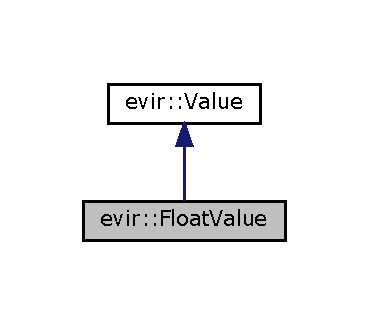
\includegraphics[width=177pt]{classevir_1_1FloatValue__inherit__graph}
\end{center}
\end{figure}


Collaboration diagram for evir\+:\+:Float\+Value\+:
\nopagebreak
\begin{figure}[H]
\begin{center}
\leavevmode
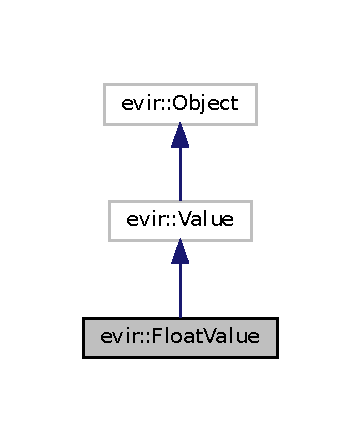
\includegraphics[width=177pt]{classevir_1_1FloatValue__coll__graph}
\end{center}
\end{figure}
\subsection*{Public Member Functions}
\begin{DoxyCompactItemize}
\item 
string \hyperlink{classevir_1_1FloatValue_a775e25d41c34aca73ed9418963bb652b}{generate\+\_\+ir} (const char $\ast$format=nullptr)
\item 
\mbox{\Hypertarget{classevir_1_1FloatValue_a99da4695fa2baf5e8b397e03dc2fca4a}\label{classevir_1_1FloatValue_a99da4695fa2baf5e8b397e03dc2fca4a}} 
{\bfseries Float\+Value} (float2 value)
\end{DoxyCompactItemize}
\subsection*{Public Attributes}
\begin{DoxyCompactItemize}
\item 
\mbox{\Hypertarget{classevir_1_1FloatValue_a15fa49462955f59082b7b1381c3867a7}\label{classevir_1_1FloatValue_a15fa49462955f59082b7b1381c3867a7}} 
float2 {\bfseries value}
\end{DoxyCompactItemize}
\subsection*{Additional Inherited Members}


\subsection{Member Function Documentation}
\mbox{\Hypertarget{classevir_1_1FloatValue_a775e25d41c34aca73ed9418963bb652b}\label{classevir_1_1FloatValue_a775e25d41c34aca73ed9418963bb652b}} 
\index{evir\+::\+Float\+Value@{evir\+::\+Float\+Value}!generate\+\_\+ir@{generate\+\_\+ir}}
\index{generate\+\_\+ir@{generate\+\_\+ir}!evir\+::\+Float\+Value@{evir\+::\+Float\+Value}}
\subsubsection{\texorpdfstring{generate\+\_\+ir()}{generate\_ir()}}
{\footnotesize\ttfamily string evir\+::\+Float\+Value\+::generate\+\_\+ir (\begin{DoxyParamCaption}\item[{const char $\ast$}]{format = {\ttfamily nullptr} }\end{DoxyParamCaption})\hspace{0.3cm}{\ttfamily [virtual]}}

Generates the IR for the value \begin{DoxyReturn}{Returns}
the IR as a string (without newline) 
\end{DoxyReturn}


Implements \hyperlink{classevir_1_1Value_a3e7e5bc634fd5bba528324076fe2a763}{evir\+::\+Value}.



The documentation for this class was generated from the following file\+:\begin{DoxyCompactItemize}
\item 
include/ir/value.\+hpp\end{DoxyCompactItemize}

\hypertarget{classevir_1_1IntegerValue}{}\doxysection{evir\+::Integer\+Value Class Reference}
\label{classevir_1_1IntegerValue}\index{evir::IntegerValue@{evir::IntegerValue}}


Inheritance diagram for evir\+::Integer\+Value\+:\nopagebreak
\begin{figure}[H]
\begin{center}
\leavevmode
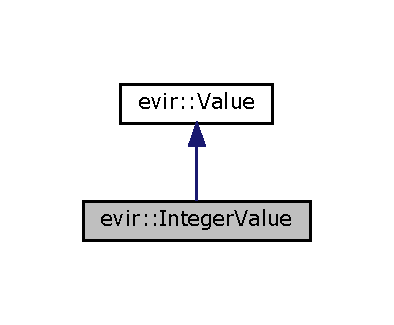
\includegraphics[width=183pt]{classevir_1_1IntegerValue__inherit__graph}
\end{center}
\end{figure}


Collaboration diagram for evir\+::Integer\+Value\+:\nopagebreak
\begin{figure}[H]
\begin{center}
\leavevmode
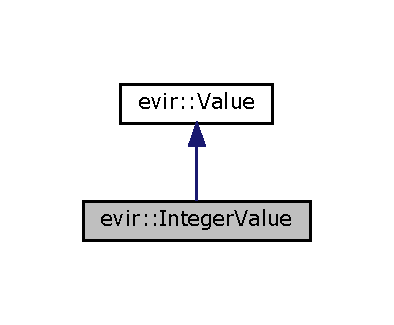
\includegraphics[width=183pt]{classevir_1_1IntegerValue__coll__graph}
\end{center}
\end{figure}
\doxysubsection*{Public Member Functions}
\begin{DoxyCompactItemize}
\item 
String \mbox{\hyperlink{classevir_1_1IntegerValue_a1c39dc084ae636a793424a125941abe0}{generate\+\_\+ir}} (const char $\ast$format=nullptr)
\item 
\mbox{\Hypertarget{classevir_1_1IntegerValue_ad22144e1c972ad4c6afab52d75049afe}\label{classevir_1_1IntegerValue_ad22144e1c972ad4c6afab52d75049afe}} 
{\bfseries Integer\+Value} (int64 value)
\end{DoxyCompactItemize}
\doxysubsection*{Public Attributes}
\begin{DoxyCompactItemize}
\item 
\mbox{\Hypertarget{classevir_1_1IntegerValue_aa93d03b5f0b6a7de8267d18de1b1774b}\label{classevir_1_1IntegerValue_aa93d03b5f0b6a7de8267d18de1b1774b}} 
int64 {\bfseries value}
\end{DoxyCompactItemize}
\doxysubsection*{Additional Inherited Members}


\doxysubsection{Member Function Documentation}
\mbox{\Hypertarget{classevir_1_1IntegerValue_a1c39dc084ae636a793424a125941abe0}\label{classevir_1_1IntegerValue_a1c39dc084ae636a793424a125941abe0}} 
\index{evir::IntegerValue@{evir::IntegerValue}!generate\_ir@{generate\_ir}}
\index{generate\_ir@{generate\_ir}!evir::IntegerValue@{evir::IntegerValue}}
\doxysubsubsection{\texorpdfstring{generate\_ir()}{generate\_ir()}}
{\footnotesize\ttfamily String evir\+::\+Integer\+Value\+::generate\+\_\+ir (\begin{DoxyParamCaption}\item[{const char $\ast$}]{format = {\ttfamily nullptr} }\end{DoxyParamCaption})\hspace{0.3cm}{\ttfamily [virtual]}}

Generates the IR for the value \begin{DoxyReturn}{Returns}
the IR as a string (without a newline) 
\end{DoxyReturn}


Implements \mbox{\hyperlink{classevir_1_1Value_a343e306225c2ba058a6caee56024d115}{evir\+::\+Value}}.



The documentation for this class was generated from the following file\+:\begin{DoxyCompactItemize}
\item 
include/ir/object/value.\+hpp\end{DoxyCompactItemize}

\hypertarget{classevir_1_1IRBuilder}{}\section{evir\+:\+:I\+R\+Builder Class Reference}
\label{classevir_1_1IRBuilder}\index{evir\+::\+I\+R\+Builder@{evir\+::\+I\+R\+Builder}}


A class for creating and managing instructions.  


\subsection*{Public Member Functions}
\begin{DoxyCompactItemize}
\item 
\mbox{\Hypertarget{classevir_1_1IRBuilder_a3d72af25adcae919d694d7bd4017e9ed}\label{classevir_1_1IRBuilder_a3d72af25adcae919d694d7bd4017e9ed}} 
\hyperlink{classevir_1_1IRBuilder_a3d72af25adcae919d694d7bd4017e9ed}{I\+R\+Builder} ()
\begin{DoxyCompactList}\small\item\em Constructs a new IR Builder. \end{DoxyCompactList}\end{DoxyCompactItemize}


\subsection{Detailed Description}
A class for creating and managing instructions. 

Instructions will be inserted in a \hyperlink{}{Basic\+Block}. ~\newline
Note that this A\+PI does not fully expose the uses of instructions. 

The documentation for this class was generated from the following file\+:\begin{DoxyCompactItemize}
\item 
include/ir/irbuilder.\+hpp\end{DoxyCompactItemize}

\hypertarget{classevir_1_1ListValue}{}\section{evir\+:\+:List\+Value Class Reference}
\label{classevir_1_1ListValue}\index{evir\+::\+List\+Value@{evir\+::\+List\+Value}}


Inheritance diagram for evir\+:\+:List\+Value\+:
\nopagebreak
\begin{figure}[H]
\begin{center}
\leavevmode
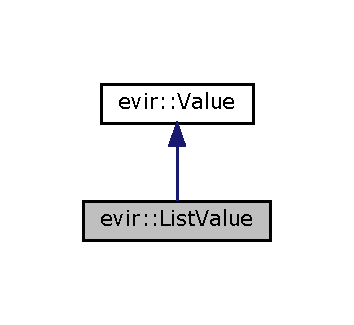
\includegraphics[width=170pt]{classevir_1_1ListValue__inherit__graph}
\end{center}
\end{figure}


Collaboration diagram for evir\+:\+:List\+Value\+:
\nopagebreak
\begin{figure}[H]
\begin{center}
\leavevmode
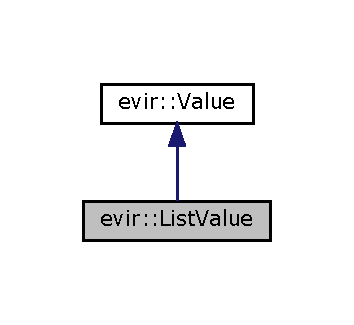
\includegraphics[width=170pt]{classevir_1_1ListValue__coll__graph}
\end{center}
\end{figure}
\subsection*{Public Member Functions}
\begin{DoxyCompactItemize}
\item 
string \hyperlink{classevir_1_1ListValue_aebd962d9117d8cd22d35bf217975dcff}{generate\+\_\+ir} (const char $\ast$format=nullptr)
\item 
\mbox{\Hypertarget{classevir_1_1ListValue_a9382018da6050ec7308d0bb6e311cc30}\label{classevir_1_1ListValue_a9382018da6050ec7308d0bb6e311cc30}} 
{\bfseries List\+Value} (vector$<$ \hyperlink{classevir_1_1Value}{Value} $\ast$$>$ elements)
\end{DoxyCompactItemize}
\subsection*{Public Attributes}
\begin{DoxyCompactItemize}
\item 
\mbox{\Hypertarget{classevir_1_1ListValue_a4b719e7544de6576a988822950be4b5c}\label{classevir_1_1ListValue_a4b719e7544de6576a988822950be4b5c}} 
vector$<$ \hyperlink{classevir_1_1Value}{Value} $\ast$ $>$ {\bfseries elements}
\end{DoxyCompactItemize}
\subsection*{Additional Inherited Members}


\subsection{Member Function Documentation}
\mbox{\Hypertarget{classevir_1_1ListValue_aebd962d9117d8cd22d35bf217975dcff}\label{classevir_1_1ListValue_aebd962d9117d8cd22d35bf217975dcff}} 
\index{evir\+::\+List\+Value@{evir\+::\+List\+Value}!generate\+\_\+ir@{generate\+\_\+ir}}
\index{generate\+\_\+ir@{generate\+\_\+ir}!evir\+::\+List\+Value@{evir\+::\+List\+Value}}
\subsubsection{\texorpdfstring{generate\+\_\+ir()}{generate\_ir()}}
{\footnotesize\ttfamily string evir\+::\+List\+Value\+::generate\+\_\+ir (\begin{DoxyParamCaption}\item[{const char $\ast$}]{format = {\ttfamily nullptr} }\end{DoxyParamCaption})\hspace{0.3cm}{\ttfamily [virtual]}}

Generates the IR for the value \begin{DoxyReturn}{Returns}
the IR as a string (without newline) 
\end{DoxyReturn}


Implements \hyperlink{classevir_1_1Value_a3e7e5bc634fd5bba528324076fe2a763}{evir\+::\+Value}.



The documentation for this class was generated from the following file\+:\begin{DoxyCompactItemize}
\item 
include/ir/value.\+hpp\end{DoxyCompactItemize}

\hypertarget{classevir_1_1Metadata}{}\doxysection{evir\+::Metadata Class Reference}
\label{classevir_1_1Metadata}\index{evir::Metadata@{evir::Metadata}}


A class defining the metadata of a \mbox{\hyperlink{classevir_1_1Module}{Module}}.  




{\ttfamily \#include $<$include/ir/metadata/metadata.\+hpp$>$}

\doxysubsection*{Public Types}
\begin{DoxyCompactItemize}
\item 
enum \mbox{\hyperlink{classevir_1_1Metadata_a12e125eae4e599760a508e21afeef02e}{Builtin\+Property\+ID}} \{ \newline
\mbox{\hyperlink{classevir_1_1Metadata_a12e125eae4e599760a508e21afeef02eaa95982da83f4bc2a85b73339c999b402}{MD\+\_\+\+MODULE\+\_\+\+NAME}}
, \newline
\mbox{\hyperlink{classevir_1_1Metadata_a12e125eae4e599760a508e21afeef02ea6f1425443e7fb11bdf2bac2327835168}{MD\+\_\+\+MODULE\+\_\+\+ENTRYPOINT}}
, \newline
\mbox{\hyperlink{classevir_1_1Metadata_a12e125eae4e599760a508e21afeef02eac53761121dca176be8ef6fa01c281db4}{MD\+\_\+\+MODULE\+\_\+\+SOURCE\+\_\+\+FILENAME}}
, \newline
\mbox{\hyperlink{classevir_1_1Metadata_a12e125eae4e599760a508e21afeef02ea55e927d6ae73aa6bbe8547b2d8cbdd95}{MD\+\_\+\+MODULE\+\_\+\+SOURCE\+\_\+\+DIRECTORY}}
, \newline
\mbox{\hyperlink{classevir_1_1Metadata_a12e125eae4e599760a508e21afeef02ea76f69addfcb4ea1c2c563ba3375d0477}{MD\+\_\+\+MODULE\+\_\+\+SOURCE\+\_\+\+LANGUAGE}}
, \newline
\mbox{\hyperlink{classevir_1_1Metadata_a12e125eae4e599760a508e21afeef02ea2c34202c27b452aa7a79aa119dfdcc8c}{MD\+\_\+\+MODULE\+\_\+\+PRODUCER\+\_\+\+NAME}}
, \newline
\mbox{\hyperlink{classevir_1_1Metadata_a12e125eae4e599760a508e21afeef02ea6169b06fa8ffb8a2947205a226b1c64f}{MD\+\_\+\+MODULE\+\_\+\+PRODUCER\+\_\+\+VERSION}}
, \newline
\mbox{\hyperlink{classevir_1_1Metadata_a12e125eae4e599760a508e21afeef02eafaf0cf5b81d7960a9544fe664939fcc4}{MD\+\_\+\+MODULE\+\_\+\+PRODUCER\+\_\+\+TYPE}}
, \newline
\mbox{\hyperlink{classevir_1_1Metadata_a12e125eae4e599760a508e21afeef02ea134fa64753dc32f743b4b52cac3b8b03}{MD\+\_\+\+TARGET\+\_\+\+TRIPLE}}
, \newline
\mbox{\hyperlink{classevir_1_1Metadata_a12e125eae4e599760a508e21afeef02ea0f18319ea7214e59f3aeaea710150f2c}{MD\+\_\+\+TARGET\+\_\+\+CPU}}
, \newline
\mbox{\hyperlink{classevir_1_1Metadata_a12e125eae4e599760a508e21afeef02ea28069d49f7f952722a4aa3aad9fcd758}{MD\+\_\+\+TARGET\+\_\+\+DATALAYOUT}}
, \newline
\mbox{\hyperlink{classevir_1_1Metadata_a12e125eae4e599760a508e21afeef02ea70aad72376f850c3c4ec8bb4bda52e9f}{MD\+\_\+\+TARGET\+\_\+\+OPTIMIZATION}}
, \newline
\mbox{\hyperlink{classevir_1_1Metadata_a12e125eae4e599760a508e21afeef02eade307a1193a25f1ac804a7527e65fb60}{MD\+\_\+\+DEBUG\+\_\+\+GENERATE}}
, \newline
\mbox{\hyperlink{classevir_1_1Metadata_a12e125eae4e599760a508e21afeef02ea90fd35626e3dee42cb50a60966e7daf7}{MD\+\_\+\+DEBUG\+\_\+\+INCLUDESOURCE}}
, \newline
\mbox{\hyperlink{classevir_1_1Metadata_a12e125eae4e599760a508e21afeef02ea0ed5bb6748ef017f4441f1add195d3cf}{MD\+\_\+\+DEBUG\+\_\+\+SOURCELOCATION}}
, \newline
\mbox{\hyperlink{classevir_1_1Metadata_a12e125eae4e599760a508e21afeef02eab848d20f8d33cff875674f665ba37099}{MD\+\_\+\+DEBUG\+\_\+\+SOURCECHECKSUM}}
, \newline
\mbox{\hyperlink{classevir_1_1Metadata_a12e125eae4e599760a508e21afeef02eacc62c019b5b4cd219f4fd00ef05566c6}{MD\+\_\+\+DEBUG\+\_\+\+DWARFVERSION}}
, \newline
\mbox{\hyperlink{classevir_1_1Metadata_a12e125eae4e599760a508e21afeef02ea0e7d4390e16e5d49f4d35bb1a7afd8b5}{MD\+\_\+\+DEBUG\+\_\+\+TYPENAMES}}
 \}
\begin{DoxyCompactList}\small\item\em built-\/in metadata property types \end{DoxyCompactList}\item 
enum \mbox{\hyperlink{classevir_1_1Metadata_a54794659073992828296c21482bb977f}{Custom\+Property\+ID}} \{ \newline
\mbox{\hyperlink{classevir_1_1Metadata_a54794659073992828296c21482bb977fa2a63ac6549ef79eadf65527a6abf6c3a}{MD\+\_\+\+MODULE}}
, \newline
\mbox{\hyperlink{classevir_1_1Metadata_a54794659073992828296c21482bb977fab18658b0a848779c775ff8f9d9654f54}{MD\+\_\+\+MODULE\+\_\+\+SOURCE}}
, \newline
\mbox{\hyperlink{classevir_1_1Metadata_a54794659073992828296c21482bb977fa1e0ddf7f85d37a24674708d6ce04f8ea}{MD\+\_\+\+MODULE\+\_\+\+PRODUCER}}
, \newline
\mbox{\hyperlink{classevir_1_1Metadata_a54794659073992828296c21482bb977fa5d744a85d597fcbd47442a1c16878cc3}{MD\+\_\+\+TARGET}}
, \newline
\mbox{\hyperlink{classevir_1_1Metadata_a54794659073992828296c21482bb977fa4cca9012ee7cf5cdbef7f60e5ed07387}{MD\+\_\+\+DEBUG}}
, \newline
\mbox{\hyperlink{classevir_1_1Metadata_a54794659073992828296c21482bb977faf5630aa6351154e62e1f49b7ee7f1549}{MD\+\_\+\+CUSTOM}}
 \}
\begin{DoxyCompactList}\small\item\em custom metadata property types \end{DoxyCompactList}\item 
\mbox{\Hypertarget{classevir_1_1Metadata_a95022cb074a6ac6d1f3c2d0e2b02ebbb}\label{classevir_1_1Metadata_a95022cb074a6ac6d1f3c2d0e2b02ebbb}} 
typedef Vector$<$ String $>$ {\bfseries Path}
\begin{DoxyCompactList}\small\item\em A metadata path. \end{DoxyCompactList}\end{DoxyCompactItemize}
\doxysubsection*{Public Member Functions}
\begin{DoxyCompactItemize}
\item 
\mbox{\hyperlink{classevir_1_1Metadata_a07e1493a76e547840d7e2a072c99e46c}{Metadata}} (\mbox{\hyperlink{classevir_1_1Metadata_a12e125eae4e599760a508e21afeef02e}{Builtin\+Property\+ID}} type, \mbox{\hyperlink{classevir_1_1MDValue}{MDValue}} $\ast$value=nullptr)
\begin{DoxyCompactList}\small\item\em Constructs a new metadata instance defining a built-\/in property. \end{DoxyCompactList}\item 
\mbox{\hyperlink{classevir_1_1Metadata_a04f985fff42ba4671f681c03e96e82f6}{Metadata}} (\mbox{\hyperlink{classevir_1_1Metadata_a54794659073992828296c21482bb977f}{Custom\+Property\+ID}} type, \mbox{\hyperlink{classevir_1_1Metadata_a95022cb074a6ac6d1f3c2d0e2b02ebbb}{Path}} path, \mbox{\hyperlink{classevir_1_1MDValue}{MDValue}} $\ast$value=nullptr)
\begin{DoxyCompactList}\small\item\em Constructs a new metadata instance defining a custom property. \end{DoxyCompactList}\item 
String \mbox{\hyperlink{classevir_1_1Metadata_ab8b6fc9bc47d7f1e8260c250ecbff96f}{generate\+\_\+ir}} ()
\begin{DoxyCompactList}\small\item\em Generates the IR for this metadata property. \end{DoxyCompactList}\end{DoxyCompactItemize}
\doxysubsection*{Static Public Member Functions}
\begin{DoxyCompactItemize}
\item 
static \mbox{\hyperlink{classevir_1_1Metadata_a95022cb074a6ac6d1f3c2d0e2b02ebbb}{Path}} \mbox{\hyperlink{classevir_1_1Metadata_a3738a45ea3dce32ebee865e7949c0233}{create\+\_\+path}} (String full\+\_\+path)
\begin{DoxyCompactList}\small\item\em Creates a Metadata path. \end{DoxyCompactList}\end{DoxyCompactItemize}


\doxysubsection{Detailed Description}
A class defining the metadata of a \mbox{\hyperlink{classevir_1_1Module}{Module}}. 

Can be added to a module using \mbox{\hyperlink{classevir_1_1Module_a8e8193a7ab86fb626058bd6135f8e2f8}{Module\+::add\+\_\+metadata}} 

\doxysubsection{Member Enumeration Documentation}
\mbox{\Hypertarget{classevir_1_1Metadata_a12e125eae4e599760a508e21afeef02e}\label{classevir_1_1Metadata_a12e125eae4e599760a508e21afeef02e}} 
\index{evir::Metadata@{evir::Metadata}!BuiltinPropertyID@{BuiltinPropertyID}}
\index{BuiltinPropertyID@{BuiltinPropertyID}!evir::Metadata@{evir::Metadata}}
\doxysubsubsection{\texorpdfstring{BuiltinPropertyID}{BuiltinPropertyID}}
{\footnotesize\ttfamily enum \mbox{\hyperlink{classevir_1_1Metadata_a12e125eae4e599760a508e21afeef02e}{evir\+::\+Metadata\+::\+Builtin\+Property\+ID}}}



built-\/in metadata property types 

Used by \mbox{\hyperlink{classevir_1_1Metadata_a07e1493a76e547840d7e2a072c99e46c}{Metadata\+::\+Metadata(\+Builtin\+Property\+ID type, MDValue$\ast$ value)}} \begin{DoxyEnumFields}{Enumerator}
\raisebox{\heightof{T}}[0pt][0pt]{\index{MD\_MODULE\_NAME@{MD\_MODULE\_NAME}!evir::Metadata@{evir::Metadata}}\index{evir::Metadata@{evir::Metadata}!MD\_MODULE\_NAME@{MD\_MODULE\_NAME}}}\mbox{\Hypertarget{classevir_1_1Metadata_a12e125eae4e599760a508e21afeef02eaa95982da83f4bc2a85b73339c999b402}\label{classevir_1_1Metadata_a12e125eae4e599760a508e21afeef02eaa95982da83f4bc2a85b73339c999b402}} 
MD\+\_\+\+MODULE\+\_\+\+NAME&metadata property path\+: {\ttfamily !module/name} \\
\hline

\raisebox{\heightof{T}}[0pt][0pt]{\index{MD\_MODULE\_ENTRYPOINT@{MD\_MODULE\_ENTRYPOINT}!evir::Metadata@{evir::Metadata}}\index{evir::Metadata@{evir::Metadata}!MD\_MODULE\_ENTRYPOINT@{MD\_MODULE\_ENTRYPOINT}}}\mbox{\Hypertarget{classevir_1_1Metadata_a12e125eae4e599760a508e21afeef02ea6f1425443e7fb11bdf2bac2327835168}\label{classevir_1_1Metadata_a12e125eae4e599760a508e21afeef02ea6f1425443e7fb11bdf2bac2327835168}} 
MD\+\_\+\+MODULE\+\_\+\+ENTRYPOINT&metadata property path\+: {\ttfamily !module/entrypoint} \\
\hline

\raisebox{\heightof{T}}[0pt][0pt]{\index{MD\_MODULE\_SOURCE\_FILENAME@{MD\_MODULE\_SOURCE\_FILENAME}!evir::Metadata@{evir::Metadata}}\index{evir::Metadata@{evir::Metadata}!MD\_MODULE\_SOURCE\_FILENAME@{MD\_MODULE\_SOURCE\_FILENAME}}}\mbox{\Hypertarget{classevir_1_1Metadata_a12e125eae4e599760a508e21afeef02eac53761121dca176be8ef6fa01c281db4}\label{classevir_1_1Metadata_a12e125eae4e599760a508e21afeef02eac53761121dca176be8ef6fa01c281db4}} 
MD\+\_\+\+MODULE\+\_\+\+SOURCE\+\_\+\+FILENAME&metadata property path\+: {\ttfamily !module/source/filename} \\
\hline

\raisebox{\heightof{T}}[0pt][0pt]{\index{MD\_MODULE\_SOURCE\_DIRECTORY@{MD\_MODULE\_SOURCE\_DIRECTORY}!evir::Metadata@{evir::Metadata}}\index{evir::Metadata@{evir::Metadata}!MD\_MODULE\_SOURCE\_DIRECTORY@{MD\_MODULE\_SOURCE\_DIRECTORY}}}\mbox{\Hypertarget{classevir_1_1Metadata_a12e125eae4e599760a508e21afeef02ea55e927d6ae73aa6bbe8547b2d8cbdd95}\label{classevir_1_1Metadata_a12e125eae4e599760a508e21afeef02ea55e927d6ae73aa6bbe8547b2d8cbdd95}} 
MD\+\_\+\+MODULE\+\_\+\+SOURCE\+\_\+\+DIRECTORY&metadata property path\+: {\ttfamily !module/source/directory} \\
\hline

\raisebox{\heightof{T}}[0pt][0pt]{\index{MD\_MODULE\_SOURCE\_LANGUAGE@{MD\_MODULE\_SOURCE\_LANGUAGE}!evir::Metadata@{evir::Metadata}}\index{evir::Metadata@{evir::Metadata}!MD\_MODULE\_SOURCE\_LANGUAGE@{MD\_MODULE\_SOURCE\_LANGUAGE}}}\mbox{\Hypertarget{classevir_1_1Metadata_a12e125eae4e599760a508e21afeef02ea76f69addfcb4ea1c2c563ba3375d0477}\label{classevir_1_1Metadata_a12e125eae4e599760a508e21afeef02ea76f69addfcb4ea1c2c563ba3375d0477}} 
MD\+\_\+\+MODULE\+\_\+\+SOURCE\+\_\+\+LANGUAGE&metadata property path\+: {\ttfamily !module/source/language} \\
\hline

\raisebox{\heightof{T}}[0pt][0pt]{\index{MD\_MODULE\_PRODUCER\_NAME@{MD\_MODULE\_PRODUCER\_NAME}!evir::Metadata@{evir::Metadata}}\index{evir::Metadata@{evir::Metadata}!MD\_MODULE\_PRODUCER\_NAME@{MD\_MODULE\_PRODUCER\_NAME}}}\mbox{\Hypertarget{classevir_1_1Metadata_a12e125eae4e599760a508e21afeef02ea2c34202c27b452aa7a79aa119dfdcc8c}\label{classevir_1_1Metadata_a12e125eae4e599760a508e21afeef02ea2c34202c27b452aa7a79aa119dfdcc8c}} 
MD\+\_\+\+MODULE\+\_\+\+PRODUCER\+\_\+\+NAME&metadata property path\+: {\ttfamily !module/producer/name} \\
\hline

\raisebox{\heightof{T}}[0pt][0pt]{\index{MD\_MODULE\_PRODUCER\_VERSION@{MD\_MODULE\_PRODUCER\_VERSION}!evir::Metadata@{evir::Metadata}}\index{evir::Metadata@{evir::Metadata}!MD\_MODULE\_PRODUCER\_VERSION@{MD\_MODULE\_PRODUCER\_VERSION}}}\mbox{\Hypertarget{classevir_1_1Metadata_a12e125eae4e599760a508e21afeef02ea6169b06fa8ffb8a2947205a226b1c64f}\label{classevir_1_1Metadata_a12e125eae4e599760a508e21afeef02ea6169b06fa8ffb8a2947205a226b1c64f}} 
MD\+\_\+\+MODULE\+\_\+\+PRODUCER\+\_\+\+VERSION&metadata property path\+: {\ttfamily !module/producer/version} \\
\hline

\raisebox{\heightof{T}}[0pt][0pt]{\index{MD\_MODULE\_PRODUCER\_TYPE@{MD\_MODULE\_PRODUCER\_TYPE}!evir::Metadata@{evir::Metadata}}\index{evir::Metadata@{evir::Metadata}!MD\_MODULE\_PRODUCER\_TYPE@{MD\_MODULE\_PRODUCER\_TYPE}}}\mbox{\Hypertarget{classevir_1_1Metadata_a12e125eae4e599760a508e21afeef02eafaf0cf5b81d7960a9544fe664939fcc4}\label{classevir_1_1Metadata_a12e125eae4e599760a508e21afeef02eafaf0cf5b81d7960a9544fe664939fcc4}} 
MD\+\_\+\+MODULE\+\_\+\+PRODUCER\+\_\+\+TYPE&metadata property path\+: {\ttfamily !module/producer/type} \\
\hline

\raisebox{\heightof{T}}[0pt][0pt]{\index{MD\_TARGET\_TRIPLE@{MD\_TARGET\_TRIPLE}!evir::Metadata@{evir::Metadata}}\index{evir::Metadata@{evir::Metadata}!MD\_TARGET\_TRIPLE@{MD\_TARGET\_TRIPLE}}}\mbox{\Hypertarget{classevir_1_1Metadata_a12e125eae4e599760a508e21afeef02ea134fa64753dc32f743b4b52cac3b8b03}\label{classevir_1_1Metadata_a12e125eae4e599760a508e21afeef02ea134fa64753dc32f743b4b52cac3b8b03}} 
MD\+\_\+\+TARGET\+\_\+\+TRIPLE&metadata property path\+: {\ttfamily !target/triple} \\
\hline

\raisebox{\heightof{T}}[0pt][0pt]{\index{MD\_TARGET\_CPU@{MD\_TARGET\_CPU}!evir::Metadata@{evir::Metadata}}\index{evir::Metadata@{evir::Metadata}!MD\_TARGET\_CPU@{MD\_TARGET\_CPU}}}\mbox{\Hypertarget{classevir_1_1Metadata_a12e125eae4e599760a508e21afeef02ea0f18319ea7214e59f3aeaea710150f2c}\label{classevir_1_1Metadata_a12e125eae4e599760a508e21afeef02ea0f18319ea7214e59f3aeaea710150f2c}} 
MD\+\_\+\+TARGET\+\_\+\+CPU&metadata property path\+: {\ttfamily !target/cpu} \\
\hline

\raisebox{\heightof{T}}[0pt][0pt]{\index{MD\_TARGET\_DATALAYOUT@{MD\_TARGET\_DATALAYOUT}!evir::Metadata@{evir::Metadata}}\index{evir::Metadata@{evir::Metadata}!MD\_TARGET\_DATALAYOUT@{MD\_TARGET\_DATALAYOUT}}}\mbox{\Hypertarget{classevir_1_1Metadata_a12e125eae4e599760a508e21afeef02ea28069d49f7f952722a4aa3aad9fcd758}\label{classevir_1_1Metadata_a12e125eae4e599760a508e21afeef02ea28069d49f7f952722a4aa3aad9fcd758}} 
MD\+\_\+\+TARGET\+\_\+\+DATALAYOUT&metadata property path\+: {\ttfamily !target/datalayout} \\
\hline

\raisebox{\heightof{T}}[0pt][0pt]{\index{MD\_TARGET\_OPTIMIZATION@{MD\_TARGET\_OPTIMIZATION}!evir::Metadata@{evir::Metadata}}\index{evir::Metadata@{evir::Metadata}!MD\_TARGET\_OPTIMIZATION@{MD\_TARGET\_OPTIMIZATION}}}\mbox{\Hypertarget{classevir_1_1Metadata_a12e125eae4e599760a508e21afeef02ea70aad72376f850c3c4ec8bb4bda52e9f}\label{classevir_1_1Metadata_a12e125eae4e599760a508e21afeef02ea70aad72376f850c3c4ec8bb4bda52e9f}} 
MD\+\_\+\+TARGET\+\_\+\+OPTIMIZATION&metadata property path\+: {\ttfamily !target/optimization} \\
\hline

\raisebox{\heightof{T}}[0pt][0pt]{\index{MD\_DEBUG\_GENERATE@{MD\_DEBUG\_GENERATE}!evir::Metadata@{evir::Metadata}}\index{evir::Metadata@{evir::Metadata}!MD\_DEBUG\_GENERATE@{MD\_DEBUG\_GENERATE}}}\mbox{\Hypertarget{classevir_1_1Metadata_a12e125eae4e599760a508e21afeef02eade307a1193a25f1ac804a7527e65fb60}\label{classevir_1_1Metadata_a12e125eae4e599760a508e21afeef02eade307a1193a25f1ac804a7527e65fb60}} 
MD\+\_\+\+DEBUG\+\_\+\+GENERATE&metadata property path\+: {\ttfamily !debug/generate} \\
\hline

\raisebox{\heightof{T}}[0pt][0pt]{\index{MD\_DEBUG\_INCLUDESOURCE@{MD\_DEBUG\_INCLUDESOURCE}!evir::Metadata@{evir::Metadata}}\index{evir::Metadata@{evir::Metadata}!MD\_DEBUG\_INCLUDESOURCE@{MD\_DEBUG\_INCLUDESOURCE}}}\mbox{\Hypertarget{classevir_1_1Metadata_a12e125eae4e599760a508e21afeef02ea90fd35626e3dee42cb50a60966e7daf7}\label{classevir_1_1Metadata_a12e125eae4e599760a508e21afeef02ea90fd35626e3dee42cb50a60966e7daf7}} 
MD\+\_\+\+DEBUG\+\_\+\+INCLUDESOURCE&metadata property path\+: {\ttfamily !debug/includesource} \\
\hline

\raisebox{\heightof{T}}[0pt][0pt]{\index{MD\_DEBUG\_SOURCELOCATION@{MD\_DEBUG\_SOURCELOCATION}!evir::Metadata@{evir::Metadata}}\index{evir::Metadata@{evir::Metadata}!MD\_DEBUG\_SOURCELOCATION@{MD\_DEBUG\_SOURCELOCATION}}}\mbox{\Hypertarget{classevir_1_1Metadata_a12e125eae4e599760a508e21afeef02ea0ed5bb6748ef017f4441f1add195d3cf}\label{classevir_1_1Metadata_a12e125eae4e599760a508e21afeef02ea0ed5bb6748ef017f4441f1add195d3cf}} 
MD\+\_\+\+DEBUG\+\_\+\+SOURCELOCATION&metadata property path\+: {\ttfamily !debug/sourcelocation} \\
\hline

\raisebox{\heightof{T}}[0pt][0pt]{\index{MD\_DEBUG\_SOURCECHECKSUM@{MD\_DEBUG\_SOURCECHECKSUM}!evir::Metadata@{evir::Metadata}}\index{evir::Metadata@{evir::Metadata}!MD\_DEBUG\_SOURCECHECKSUM@{MD\_DEBUG\_SOURCECHECKSUM}}}\mbox{\Hypertarget{classevir_1_1Metadata_a12e125eae4e599760a508e21afeef02eab848d20f8d33cff875674f665ba37099}\label{classevir_1_1Metadata_a12e125eae4e599760a508e21afeef02eab848d20f8d33cff875674f665ba37099}} 
MD\+\_\+\+DEBUG\+\_\+\+SOURCECHECKSUM&metadata property path\+: {\ttfamily !debug/sourcechecksum} \\
\hline

\raisebox{\heightof{T}}[0pt][0pt]{\index{MD\_DEBUG\_DWARFVERSION@{MD\_DEBUG\_DWARFVERSION}!evir::Metadata@{evir::Metadata}}\index{evir::Metadata@{evir::Metadata}!MD\_DEBUG\_DWARFVERSION@{MD\_DEBUG\_DWARFVERSION}}}\mbox{\Hypertarget{classevir_1_1Metadata_a12e125eae4e599760a508e21afeef02eacc62c019b5b4cd219f4fd00ef05566c6}\label{classevir_1_1Metadata_a12e125eae4e599760a508e21afeef02eacc62c019b5b4cd219f4fd00ef05566c6}} 
MD\+\_\+\+DEBUG\+\_\+\+DWARFVERSION&metadata property path\+: {\ttfamily !debug/dwarfversion} \\
\hline

\raisebox{\heightof{T}}[0pt][0pt]{\index{MD\_DEBUG\_TYPENAMES@{MD\_DEBUG\_TYPENAMES}!evir::Metadata@{evir::Metadata}}\index{evir::Metadata@{evir::Metadata}!MD\_DEBUG\_TYPENAMES@{MD\_DEBUG\_TYPENAMES}}}\mbox{\Hypertarget{classevir_1_1Metadata_a12e125eae4e599760a508e21afeef02ea0e7d4390e16e5d49f4d35bb1a7afd8b5}\label{classevir_1_1Metadata_a12e125eae4e599760a508e21afeef02ea0e7d4390e16e5d49f4d35bb1a7afd8b5}} 
MD\+\_\+\+DEBUG\+\_\+\+TYPENAMES&metadata property path\+: {\ttfamily !debug/typenames} \\
\hline

\end{DoxyEnumFields}
\mbox{\Hypertarget{classevir_1_1Metadata_a54794659073992828296c21482bb977f}\label{classevir_1_1Metadata_a54794659073992828296c21482bb977f}} 
\index{evir::Metadata@{evir::Metadata}!CustomPropertyID@{CustomPropertyID}}
\index{CustomPropertyID@{CustomPropertyID}!evir::Metadata@{evir::Metadata}}
\doxysubsubsection{\texorpdfstring{CustomPropertyID}{CustomPropertyID}}
{\footnotesize\ttfamily enum \mbox{\hyperlink{classevir_1_1Metadata_a54794659073992828296c21482bb977f}{evir\+::\+Metadata\+::\+Custom\+Property\+ID}}}



custom metadata property types 

Used by \mbox{\hyperlink{classevir_1_1Metadata_a04f985fff42ba4671f681c03e96e82f6}{Metadata\+::\+Metadata(\+Custom\+Property\+ID type, Path path, MDValue$\ast$ value)}} \begin{DoxyEnumFields}{Enumerator}
\raisebox{\heightof{T}}[0pt][0pt]{\index{MD\_MODULE@{MD\_MODULE}!evir::Metadata@{evir::Metadata}}\index{evir::Metadata@{evir::Metadata}!MD\_MODULE@{MD\_MODULE}}}\mbox{\Hypertarget{classevir_1_1Metadata_a54794659073992828296c21482bb977fa2a63ac6549ef79eadf65527a6abf6c3a}\label{classevir_1_1Metadata_a54794659073992828296c21482bb977fa2a63ac6549ef79eadf65527a6abf6c3a}} 
MD\+\_\+\+MODULE&metadata property path\+: {\ttfamily !module/...} \\
\hline

\raisebox{\heightof{T}}[0pt][0pt]{\index{MD\_MODULE\_SOURCE@{MD\_MODULE\_SOURCE}!evir::Metadata@{evir::Metadata}}\index{evir::Metadata@{evir::Metadata}!MD\_MODULE\_SOURCE@{MD\_MODULE\_SOURCE}}}\mbox{\Hypertarget{classevir_1_1Metadata_a54794659073992828296c21482bb977fab18658b0a848779c775ff8f9d9654f54}\label{classevir_1_1Metadata_a54794659073992828296c21482bb977fab18658b0a848779c775ff8f9d9654f54}} 
MD\+\_\+\+MODULE\+\_\+\+SOURCE&metadata property path\+: {\ttfamily !module/source/...} \\
\hline

\raisebox{\heightof{T}}[0pt][0pt]{\index{MD\_MODULE\_PRODUCER@{MD\_MODULE\_PRODUCER}!evir::Metadata@{evir::Metadata}}\index{evir::Metadata@{evir::Metadata}!MD\_MODULE\_PRODUCER@{MD\_MODULE\_PRODUCER}}}\mbox{\Hypertarget{classevir_1_1Metadata_a54794659073992828296c21482bb977fa1e0ddf7f85d37a24674708d6ce04f8ea}\label{classevir_1_1Metadata_a54794659073992828296c21482bb977fa1e0ddf7f85d37a24674708d6ce04f8ea}} 
MD\+\_\+\+MODULE\+\_\+\+PRODUCER&metadata property path\+: {\ttfamily !module/producer/...} \\
\hline

\raisebox{\heightof{T}}[0pt][0pt]{\index{MD\_TARGET@{MD\_TARGET}!evir::Metadata@{evir::Metadata}}\index{evir::Metadata@{evir::Metadata}!MD\_TARGET@{MD\_TARGET}}}\mbox{\Hypertarget{classevir_1_1Metadata_a54794659073992828296c21482bb977fa5d744a85d597fcbd47442a1c16878cc3}\label{classevir_1_1Metadata_a54794659073992828296c21482bb977fa5d744a85d597fcbd47442a1c16878cc3}} 
MD\+\_\+\+TARGET&metadata property path\+: {\ttfamily !target/...} \\
\hline

\raisebox{\heightof{T}}[0pt][0pt]{\index{MD\_DEBUG@{MD\_DEBUG}!evir::Metadata@{evir::Metadata}}\index{evir::Metadata@{evir::Metadata}!MD\_DEBUG@{MD\_DEBUG}}}\mbox{\Hypertarget{classevir_1_1Metadata_a54794659073992828296c21482bb977fa4cca9012ee7cf5cdbef7f60e5ed07387}\label{classevir_1_1Metadata_a54794659073992828296c21482bb977fa4cca9012ee7cf5cdbef7f60e5ed07387}} 
MD\+\_\+\+DEBUG&metadata property path\+: {\ttfamily !debug/...} \\
\hline

\raisebox{\heightof{T}}[0pt][0pt]{\index{MD\_CUSTOM@{MD\_CUSTOM}!evir::Metadata@{evir::Metadata}}\index{evir::Metadata@{evir::Metadata}!MD\_CUSTOM@{MD\_CUSTOM}}}\mbox{\Hypertarget{classevir_1_1Metadata_a54794659073992828296c21482bb977faf5630aa6351154e62e1f49b7ee7f1549}\label{classevir_1_1Metadata_a54794659073992828296c21482bb977faf5630aa6351154e62e1f49b7ee7f1549}} 
MD\+\_\+\+CUSTOM&metadata property path\+: {\ttfamily !...} \\
\hline

\end{DoxyEnumFields}


\doxysubsection{Constructor \& Destructor Documentation}
\mbox{\Hypertarget{classevir_1_1Metadata_a07e1493a76e547840d7e2a072c99e46c}\label{classevir_1_1Metadata_a07e1493a76e547840d7e2a072c99e46c}} 
\index{evir::Metadata@{evir::Metadata}!Metadata@{Metadata}}
\index{Metadata@{Metadata}!evir::Metadata@{evir::Metadata}}
\doxysubsubsection{\texorpdfstring{Metadata()}{Metadata()}\hspace{0.1cm}{\footnotesize\ttfamily [1/2]}}
{\footnotesize\ttfamily evir\+::\+Metadata\+::\+Metadata (\begin{DoxyParamCaption}\item[{\mbox{\hyperlink{classevir_1_1Metadata_a12e125eae4e599760a508e21afeef02e}{Builtin\+Property\+ID}}}]{type,  }\item[{\mbox{\hyperlink{classevir_1_1MDValue}{MDValue}} $\ast$}]{value = {\ttfamily nullptr} }\end{DoxyParamCaption})}



Constructs a new metadata instance defining a built-\/in property. 


\begin{DoxyParams}{Parameters}
{\em type} & the built-\/in property type that this metadata defines \\
\hline
{\em value} & the value of this metadata property \\
\hline
\end{DoxyParams}
\mbox{\Hypertarget{classevir_1_1Metadata_a04f985fff42ba4671f681c03e96e82f6}\label{classevir_1_1Metadata_a04f985fff42ba4671f681c03e96e82f6}} 
\index{evir::Metadata@{evir::Metadata}!Metadata@{Metadata}}
\index{Metadata@{Metadata}!evir::Metadata@{evir::Metadata}}
\doxysubsubsection{\texorpdfstring{Metadata()}{Metadata()}\hspace{0.1cm}{\footnotesize\ttfamily [2/2]}}
{\footnotesize\ttfamily evir\+::\+Metadata\+::\+Metadata (\begin{DoxyParamCaption}\item[{\mbox{\hyperlink{classevir_1_1Metadata_a54794659073992828296c21482bb977f}{Custom\+Property\+ID}}}]{type,  }\item[{\mbox{\hyperlink{classevir_1_1Metadata_a95022cb074a6ac6d1f3c2d0e2b02ebbb}{Path}}}]{path,  }\item[{\mbox{\hyperlink{classevir_1_1MDValue}{MDValue}} $\ast$}]{value = {\ttfamily nullptr} }\end{DoxyParamCaption})}



Constructs a new metadata instance defining a custom property. 


\begin{DoxyParams}{Parameters}
{\em type} & the built-\/in type that this metadata defines a property of \\
\hline
{\em path} & the rest of the path of the property that this metadata defines \\
\hline
{\em value} & the value of this metadata property \\
\hline
\end{DoxyParams}


\doxysubsection{Member Function Documentation}
\mbox{\Hypertarget{classevir_1_1Metadata_a3738a45ea3dce32ebee865e7949c0233}\label{classevir_1_1Metadata_a3738a45ea3dce32ebee865e7949c0233}} 
\index{evir::Metadata@{evir::Metadata}!create\_path@{create\_path}}
\index{create\_path@{create\_path}!evir::Metadata@{evir::Metadata}}
\doxysubsubsection{\texorpdfstring{create\_path()}{create\_path()}}
{\footnotesize\ttfamily static \mbox{\hyperlink{classevir_1_1Metadata_a95022cb074a6ac6d1f3c2d0e2b02ebbb}{Path}} evir\+::\+Metadata\+::create\+\_\+path (\begin{DoxyParamCaption}\item[{String}]{full\+\_\+path }\end{DoxyParamCaption})\hspace{0.3cm}{\ttfamily [static]}}



Creates a Metadata path. 

Splits the given string into segments using {\ttfamily /} delimeters and returns that as a path 
\begin{DoxyParams}{Parameters}
{\em full\+\_\+path} & the path to use (e.\+g. \char`\"{}base/sub\char`\"{}) \\
\hline
\end{DoxyParams}
\mbox{\Hypertarget{classevir_1_1Metadata_ab8b6fc9bc47d7f1e8260c250ecbff96f}\label{classevir_1_1Metadata_ab8b6fc9bc47d7f1e8260c250ecbff96f}} 
\index{evir::Metadata@{evir::Metadata}!generate\_ir@{generate\_ir}}
\index{generate\_ir@{generate\_ir}!evir::Metadata@{evir::Metadata}}
\doxysubsubsection{\texorpdfstring{generate\_ir()}{generate\_ir()}}
{\footnotesize\ttfamily String evir\+::\+Metadata\+::generate\+\_\+ir (\begin{DoxyParamCaption}{ }\end{DoxyParamCaption})}



Generates the IR for this metadata property. 

\begin{DoxyReturn}{Returns}
the ir as a string (without a newline) 
\end{DoxyReturn}


The documentation for this class was generated from the following file\+:\begin{DoxyCompactItemize}
\item 
include/ir/metadata/metadata.\+hpp\end{DoxyCompactItemize}

\hypertarget{classevir_1_1Module}{}\doxysection{evir\+::Module Class Reference}
\label{classevir_1_1Module}\index{evir::Module@{evir::Module}}


A Class representing a single stand-\/alone IR module.  




{\ttfamily \#include $<$include/ir/module.\+hpp$>$}

\doxysubsection*{Public Member Functions}
\begin{DoxyCompactItemize}
\item 
\mbox{\Hypertarget{classevir_1_1Module_a7c323d88c85f42b4cc4824cbae0db2fe}\label{classevir_1_1Module_a7c323d88c85f42b4cc4824cbae0db2fe}} 
{\bfseries Module} ()
\begin{DoxyCompactList}\small\item\em Constructs a new module. \end{DoxyCompactList}\item 
\mbox{\hyperlink{classevir_1_1Module_a9d8a3459011354b49ee984fa52b6c4d9}{Module}} (String module\+\_\+name)
\begin{DoxyCompactList}\small\item\em Constructs a new module. \end{DoxyCompactList}\item 
String \mbox{\hyperlink{classevir_1_1Module_a154991c8367ffe72899c59e79a00941f}{get\+\_\+name}} ()
\item 
\mbox{\Hypertarget{classevir_1_1Module_a2b53dfd4cbb4228e26394bdff9725552}\label{classevir_1_1Module_a2b53dfd4cbb4228e26394bdff9725552}} 
bool {\bfseries has\+\_\+metadata} (\mbox{\hyperlink{classevir_1_1Metadata_a95022cb074a6ac6d1f3c2d0e2b02ebbb}{Metadata\+::\+Path}} path)
\begin{DoxyCompactList}\small\item\em Checks if the module has metadata with the given path. \end{DoxyCompactList}\item 
\mbox{\Hypertarget{classevir_1_1Module_aeb178190f52430e9a6a5fcceae09d2e5}\label{classevir_1_1Module_aeb178190f52430e9a6a5fcceae09d2e5}} 
bool {\bfseries has\+\_\+metadata} (\mbox{\hyperlink{classevir_1_1Metadata_a12e125eae4e599760a508e21afeef02e}{Metadata\+::\+Builtin\+Property\+ID}} type)
\begin{DoxyCompactList}\small\item\em Checks if the module has metadata with the given type. \end{DoxyCompactList}\item 
void \mbox{\hyperlink{classevir_1_1Module_a8e8193a7ab86fb626058bd6135f8e2f8}{add\+\_\+metadata}} (\mbox{\hyperlink{classevir_1_1Metadata}{Metadata}} $\ast$mdata)
\begin{DoxyCompactList}\small\item\em Adds metadata to the module. \end{DoxyCompactList}\item 
void \mbox{\hyperlink{classevir_1_1Module_af8764ad3e44a8fe939439a2bf1544986}{add\+\_\+metadata}} (\mbox{\hyperlink{classevir_1_1Metadata_a12e125eae4e599760a508e21afeef02e}{Metadata\+::\+Builtin\+Property\+ID}} id, \mbox{\hyperlink{classevir_1_1MDValue}{MDValue}} $\ast$value)
\begin{DoxyCompactList}\small\item\em Adds metadata to the module. \end{DoxyCompactList}\item 
void \mbox{\hyperlink{classevir_1_1Module_a8077df8d0dd3bebeab4cb940ec266664}{set\+\_\+metadata}} (\mbox{\hyperlink{classevir_1_1Metadata_a95022cb074a6ac6d1f3c2d0e2b02ebbb}{Metadata\+::\+Path}} path, \mbox{\hyperlink{classevir_1_1MDValue}{MDValue}} $\ast$value)
\begin{DoxyCompactList}\small\item\em Sets a metadata property with the given path. \end{DoxyCompactList}\item 
void \mbox{\hyperlink{classevir_1_1Module_a3c358833678977212573c10e7b4c618e}{set\+\_\+metadata}} (\mbox{\hyperlink{classevir_1_1Metadata_a12e125eae4e599760a508e21afeef02e}{Metadata\+::\+Builtin\+Property\+ID}} type, \mbox{\hyperlink{classevir_1_1MDValue}{MDValue}} $\ast$value)
\begin{DoxyCompactList}\small\item\em Sets a metadata property with the built-\/in type. \end{DoxyCompactList}\item 
\mbox{\hyperlink{classevir_1_1Metadata}{Metadata}} $\ast$ \mbox{\hyperlink{classevir_1_1Module_afd44eb8d5ae737998cdf4d8a9fa6fc0c}{get\+\_\+metadata}} (\mbox{\hyperlink{classevir_1_1Metadata_a95022cb074a6ac6d1f3c2d0e2b02ebbb}{Metadata\+::\+Path}} path)
\begin{DoxyCompactList}\small\item\em Gets the requested metadata property. \end{DoxyCompactList}\item 
\mbox{\hyperlink{classevir_1_1Metadata}{Metadata}} $\ast$ \mbox{\hyperlink{classevir_1_1Module_a7931a66d927c09b11e4e501aa3248102}{get\+\_\+metadata}} (\mbox{\hyperlink{classevir_1_1Metadata_a12e125eae4e599760a508e21afeef02e}{Metadata\+::\+Builtin\+Property\+ID}} type)
\begin{DoxyCompactList}\small\item\em Gets the requested metadata property. \end{DoxyCompactList}\item 
\mbox{\hyperlink{classevir_1_1Function}{Function}} $\ast$ \mbox{\hyperlink{classevir_1_1Module_a795e30b2d6f8af2b21a6f9767cf62b77}{get\+\_\+function}} (String name)
\item 
\mbox{\hyperlink{classevir_1_1Function}{Function}} $\ast$ \mbox{\hyperlink{classevir_1_1Module_ac3bace1007f3a14fb0b01ab77b47a473}{get\+\_\+or\+\_\+insert\+\_\+function}} (\mbox{\hyperlink{classevir_1_1FunctionType}{Function\+Type}} $\ast$type, String name)
\item 
String \mbox{\hyperlink{classevir_1_1Module_af713049800faeb4aea0ae91c580c5c52}{generate\+\_\+metadata\+\_\+ir}} (bool before\+\_\+contents)
\begin{DoxyCompactList}\small\item\em Generates the IR of the current module\textquotesingle{}s metadata. \end{DoxyCompactList}\item 
String \mbox{\hyperlink{classevir_1_1Module_a938af35989bf5221fd3fb8d0cff51586}{generate\+\_\+ir}} ()
\begin{DoxyCompactList}\small\item\em Generates the IR of the current module. \end{DoxyCompactList}\end{DoxyCompactItemize}


\doxysubsection{Detailed Description}
A Class representing a single stand-\/alone IR module. 

Has the following metadata by default\+:
\begin{DoxyItemize}
\item \mbox{\hyperlink{classevir_1_1Metadata_a12e125eae4e599760a508e21afeef02e}{Metadata\+::\+Builtin\+Property\+ID}}\+::{\ttfamily META\+\_\+\+MODULE\+\_\+\+NAME}
\item \mbox{\hyperlink{classevir_1_1Metadata_a12e125eae4e599760a508e21afeef02e}{Metadata\+::\+Builtin\+Property\+ID}}\+::{\ttfamily META\+\_\+\+MODULE\+\_\+\+ENTRYPOINT} ~\newline
 
\end{DoxyItemize}

\doxysubsection{Constructor \& Destructor Documentation}
\mbox{\Hypertarget{classevir_1_1Module_a9d8a3459011354b49ee984fa52b6c4d9}\label{classevir_1_1Module_a9d8a3459011354b49ee984fa52b6c4d9}} 
\index{evir::Module@{evir::Module}!Module@{Module}}
\index{Module@{Module}!evir::Module@{evir::Module}}
\doxysubsubsection{\texorpdfstring{Module()}{Module()}}
{\footnotesize\ttfamily evir\+::\+Module\+::\+Module (\begin{DoxyParamCaption}\item[{String}]{module\+\_\+name }\end{DoxyParamCaption})}



Constructs a new module. 


\begin{DoxyParams}{Parameters}
{\em module\+\_\+name} & the name of the module \\
\hline
\end{DoxyParams}


\doxysubsection{Member Function Documentation}
\mbox{\Hypertarget{classevir_1_1Module_a8e8193a7ab86fb626058bd6135f8e2f8}\label{classevir_1_1Module_a8e8193a7ab86fb626058bd6135f8e2f8}} 
\index{evir::Module@{evir::Module}!add\_metadata@{add\_metadata}}
\index{add\_metadata@{add\_metadata}!evir::Module@{evir::Module}}
\doxysubsubsection{\texorpdfstring{add\_metadata()}{add\_metadata()}\hspace{0.1cm}{\footnotesize\ttfamily [1/2]}}
{\footnotesize\ttfamily void evir\+::\+Module\+::add\+\_\+metadata (\begin{DoxyParamCaption}\item[{\mbox{\hyperlink{classevir_1_1Metadata}{Metadata}} $\ast$}]{mdata }\end{DoxyParamCaption})}



Adds metadata to the module. 


\begin{DoxyParams}{Parameters}
{\em mdata} & the metadata to add \\
\hline
\end{DoxyParams}
\begin{DoxyWarning}{Warning}
if the module already has metadata with the same path the function will abort 
\end{DoxyWarning}
\mbox{\Hypertarget{classevir_1_1Module_af8764ad3e44a8fe939439a2bf1544986}\label{classevir_1_1Module_af8764ad3e44a8fe939439a2bf1544986}} 
\index{evir::Module@{evir::Module}!add\_metadata@{add\_metadata}}
\index{add\_metadata@{add\_metadata}!evir::Module@{evir::Module}}
\doxysubsubsection{\texorpdfstring{add\_metadata()}{add\_metadata()}\hspace{0.1cm}{\footnotesize\ttfamily [2/2]}}
{\footnotesize\ttfamily void evir\+::\+Module\+::add\+\_\+metadata (\begin{DoxyParamCaption}\item[{\mbox{\hyperlink{classevir_1_1Metadata_a12e125eae4e599760a508e21afeef02e}{Metadata\+::\+Builtin\+Property\+ID}}}]{id,  }\item[{\mbox{\hyperlink{classevir_1_1MDValue}{MDValue}} $\ast$}]{value }\end{DoxyParamCaption})}



Adds metadata to the module. 


\begin{DoxyParams}{Parameters}
{\em id} & the id of the builtin property to add \\
\hline
{\em value} & the value of the metadata \\
\hline
\end{DoxyParams}
\begin{DoxyWarning}{Warning}
if the module already has metadata with the same path the function will abort 
\end{DoxyWarning}
\mbox{\Hypertarget{classevir_1_1Module_a938af35989bf5221fd3fb8d0cff51586}\label{classevir_1_1Module_a938af35989bf5221fd3fb8d0cff51586}} 
\index{evir::Module@{evir::Module}!generate\_ir@{generate\_ir}}
\index{generate\_ir@{generate\_ir}!evir::Module@{evir::Module}}
\doxysubsubsection{\texorpdfstring{generate\_ir()}{generate\_ir()}}
{\footnotesize\ttfamily String evir\+::\+Module\+::generate\+\_\+ir (\begin{DoxyParamCaption}{ }\end{DoxyParamCaption})}



Generates the IR of the current module. 

\begin{DoxyReturn}{Returns}
the IR as a string (with newline) 
\end{DoxyReturn}
\mbox{\Hypertarget{classevir_1_1Module_af713049800faeb4aea0ae91c580c5c52}\label{classevir_1_1Module_af713049800faeb4aea0ae91c580c5c52}} 
\index{evir::Module@{evir::Module}!generate\_metadata\_ir@{generate\_metadata\_ir}}
\index{generate\_metadata\_ir@{generate\_metadata\_ir}!evir::Module@{evir::Module}}
\doxysubsubsection{\texorpdfstring{generate\_metadata\_ir()}{generate\_metadata\_ir()}}
{\footnotesize\ttfamily String evir\+::\+Module\+::generate\+\_\+metadata\+\_\+ir (\begin{DoxyParamCaption}\item[{bool}]{before\+\_\+contents }\end{DoxyParamCaption})}



Generates the IR of the current module\textquotesingle{}s metadata. 

If before\+\_\+contents is true, the metadata that comes before the module\textquotesingle{}s is generated, otherwise the metadata that comes after the module\textquotesingle{}s contents is generated 
\begin{DoxyParams}{Parameters}
{\em before\+\_\+contents} & see description \\
\hline
\end{DoxyParams}
\begin{DoxyReturn}{Returns}
the IR as a string (with newline) 
\end{DoxyReturn}
\mbox{\Hypertarget{classevir_1_1Module_a795e30b2d6f8af2b21a6f9767cf62b77}\label{classevir_1_1Module_a795e30b2d6f8af2b21a6f9767cf62b77}} 
\index{evir::Module@{evir::Module}!get\_function@{get\_function}}
\index{get\_function@{get\_function}!evir::Module@{evir::Module}}
\doxysubsubsection{\texorpdfstring{get\_function()}{get\_function()}}
{\footnotesize\ttfamily \mbox{\hyperlink{classevir_1_1Function}{Function}} $\ast$ evir\+::\+Module\+::get\+\_\+function (\begin{DoxyParamCaption}\item[{String}]{name }\end{DoxyParamCaption})}

\begin{DoxyReturn}{Returns}
The function if it exists, otherwise a nullptr 
\end{DoxyReturn}
\mbox{\Hypertarget{classevir_1_1Module_a7931a66d927c09b11e4e501aa3248102}\label{classevir_1_1Module_a7931a66d927c09b11e4e501aa3248102}} 
\index{evir::Module@{evir::Module}!get\_metadata@{get\_metadata}}
\index{get\_metadata@{get\_metadata}!evir::Module@{evir::Module}}
\doxysubsubsection{\texorpdfstring{get\_metadata()}{get\_metadata()}\hspace{0.1cm}{\footnotesize\ttfamily [1/2]}}
{\footnotesize\ttfamily \mbox{\hyperlink{classevir_1_1Metadata}{Metadata}} $\ast$ evir\+::\+Module\+::get\+\_\+metadata (\begin{DoxyParamCaption}\item[{\mbox{\hyperlink{classevir_1_1Metadata_a12e125eae4e599760a508e21afeef02e}{Metadata\+::\+Builtin\+Property\+ID}}}]{type }\end{DoxyParamCaption})}



Gets the requested metadata property. 


\begin{DoxyParams}{Parameters}
{\em type} & the built-\/in type of the metadata property \\
\hline
\end{DoxyParams}
\begin{DoxyReturn}{Returns}
a pointer to the metadata, or null if it isn\textquotesingle{}t found 
\end{DoxyReturn}
\mbox{\Hypertarget{classevir_1_1Module_afd44eb8d5ae737998cdf4d8a9fa6fc0c}\label{classevir_1_1Module_afd44eb8d5ae737998cdf4d8a9fa6fc0c}} 
\index{evir::Module@{evir::Module}!get\_metadata@{get\_metadata}}
\index{get\_metadata@{get\_metadata}!evir::Module@{evir::Module}}
\doxysubsubsection{\texorpdfstring{get\_metadata()}{get\_metadata()}\hspace{0.1cm}{\footnotesize\ttfamily [2/2]}}
{\footnotesize\ttfamily \mbox{\hyperlink{classevir_1_1Metadata}{Metadata}} $\ast$ evir\+::\+Module\+::get\+\_\+metadata (\begin{DoxyParamCaption}\item[{\mbox{\hyperlink{classevir_1_1Metadata_a95022cb074a6ac6d1f3c2d0e2b02ebbb}{Metadata\+::\+Path}}}]{path }\end{DoxyParamCaption})}



Gets the requested metadata property. 


\begin{DoxyParams}{Parameters}
{\em path} & the path of the metadata property \\
\hline
\end{DoxyParams}
\begin{DoxyReturn}{Returns}
a pointer to the metadata, or null if it isn\textquotesingle{}t found 
\end{DoxyReturn}
\mbox{\Hypertarget{classevir_1_1Module_a154991c8367ffe72899c59e79a00941f}\label{classevir_1_1Module_a154991c8367ffe72899c59e79a00941f}} 
\index{evir::Module@{evir::Module}!get\_name@{get\_name}}
\index{get\_name@{get\_name}!evir::Module@{evir::Module}}
\doxysubsubsection{\texorpdfstring{get\_name()}{get\_name()}}
{\footnotesize\ttfamily String evir\+::\+Module\+::get\+\_\+name (\begin{DoxyParamCaption}{ }\end{DoxyParamCaption})}

\begin{DoxyReturn}{Returns}
The name of the module if set properly, 

otherwise an empty string. 
\end{DoxyReturn}
\mbox{\Hypertarget{classevir_1_1Module_ac3bace1007f3a14fb0b01ab77b47a473}\label{classevir_1_1Module_ac3bace1007f3a14fb0b01ab77b47a473}} 
\index{evir::Module@{evir::Module}!get\_or\_insert\_function@{get\_or\_insert\_function}}
\index{get\_or\_insert\_function@{get\_or\_insert\_function}!evir::Module@{evir::Module}}
\doxysubsubsection{\texorpdfstring{get\_or\_insert\_function()}{get\_or\_insert\_function()}}
{\footnotesize\ttfamily \mbox{\hyperlink{classevir_1_1Function}{Function}} $\ast$ evir\+::\+Module\+::get\+\_\+or\+\_\+insert\+\_\+function (\begin{DoxyParamCaption}\item[{\mbox{\hyperlink{classevir_1_1FunctionType}{Function\+Type}} $\ast$}]{type,  }\item[{String}]{name }\end{DoxyParamCaption})}

\begin{DoxyReturn}{Returns}
The function if it exists, or a new function 

if it doesn\textquotesingle{}t. A nullptr is returned if a user 

with the same name exists with a different type. 
\end{DoxyReturn}
\mbox{\Hypertarget{classevir_1_1Module_a3c358833678977212573c10e7b4c618e}\label{classevir_1_1Module_a3c358833678977212573c10e7b4c618e}} 
\index{evir::Module@{evir::Module}!set\_metadata@{set\_metadata}}
\index{set\_metadata@{set\_metadata}!evir::Module@{evir::Module}}
\doxysubsubsection{\texorpdfstring{set\_metadata()}{set\_metadata()}\hspace{0.1cm}{\footnotesize\ttfamily [1/2]}}
{\footnotesize\ttfamily void evir\+::\+Module\+::set\+\_\+metadata (\begin{DoxyParamCaption}\item[{\mbox{\hyperlink{classevir_1_1Metadata_a12e125eae4e599760a508e21afeef02e}{Metadata\+::\+Builtin\+Property\+ID}}}]{type,  }\item[{\mbox{\hyperlink{classevir_1_1MDValue}{MDValue}} $\ast$}]{value }\end{DoxyParamCaption})}



Sets a metadata property with the built-\/in type. 


\begin{DoxyParams}{Parameters}
{\em type} & the type of the metadata property \\
\hline
{\em value} & the value to set the property to \\
\hline
\end{DoxyParams}
\begin{DoxyWarning}{Warning}
if the module doesn\textquotesingle{}t have metadata with the given type the function will abort 
\end{DoxyWarning}
\mbox{\Hypertarget{classevir_1_1Module_a8077df8d0dd3bebeab4cb940ec266664}\label{classevir_1_1Module_a8077df8d0dd3bebeab4cb940ec266664}} 
\index{evir::Module@{evir::Module}!set\_metadata@{set\_metadata}}
\index{set\_metadata@{set\_metadata}!evir::Module@{evir::Module}}
\doxysubsubsection{\texorpdfstring{set\_metadata()}{set\_metadata()}\hspace{0.1cm}{\footnotesize\ttfamily [2/2]}}
{\footnotesize\ttfamily void evir\+::\+Module\+::set\+\_\+metadata (\begin{DoxyParamCaption}\item[{\mbox{\hyperlink{classevir_1_1Metadata_a95022cb074a6ac6d1f3c2d0e2b02ebbb}{Metadata\+::\+Path}}}]{path,  }\item[{\mbox{\hyperlink{classevir_1_1MDValue}{MDValue}} $\ast$}]{value }\end{DoxyParamCaption})}



Sets a metadata property with the given path. 


\begin{DoxyParams}{Parameters}
{\em path} & the path of the metadata property \\
\hline
{\em value} & the value to set the property to \\
\hline
\end{DoxyParams}
\begin{DoxyWarning}{Warning}
if the module doesn\textquotesingle{}t have metadata with the given path the function will abort 
\end{DoxyWarning}


The documentation for this class was generated from the following file\+:\begin{DoxyCompactItemize}
\item 
include/ir/module.\+hpp\end{DoxyCompactItemize}

\hypertarget{classevir_1_1ObjectValue}{}\section{evir\+:\+:Object\+Value Class Reference}
\label{classevir_1_1ObjectValue}\index{evir\+::\+Object\+Value@{evir\+::\+Object\+Value}}


Inheritance diagram for evir\+:\+:Object\+Value\+:
\nopagebreak
\begin{figure}[H]
\begin{center}
\leavevmode
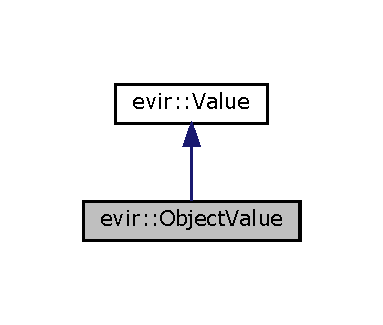
\includegraphics[width=184pt]{classevir_1_1ObjectValue__inherit__graph}
\end{center}
\end{figure}


Collaboration diagram for evir\+:\+:Object\+Value\+:
\nopagebreak
\begin{figure}[H]
\begin{center}
\leavevmode
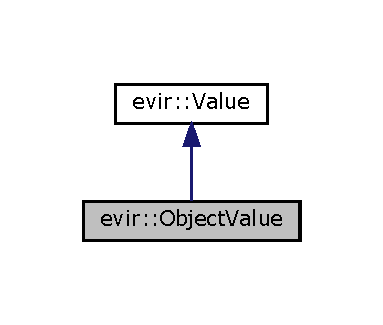
\includegraphics[width=184pt]{classevir_1_1ObjectValue__coll__graph}
\end{center}
\end{figure}
\subsection*{Public Member Functions}
\begin{DoxyCompactItemize}
\item 
string \hyperlink{classevir_1_1ObjectValue_a1058f47731ab800327893e388fc2b2d0}{generate\+\_\+ir} (const char $\ast$format=nullptr)
\item 
\mbox{\Hypertarget{classevir_1_1ObjectValue_aa73660ddf07e9428f8758c370b66c604}\label{classevir_1_1ObjectValue_aa73660ddf07e9428f8758c370b66c604}} 
{\bfseries Object\+Value} (map$<$ \hyperlink{classevir_1_1Value}{Value} $\ast$C\+O\+M\+MA \hyperlink{classevir_1_1Value}{Value} $\ast$$>$ pairs)
\end{DoxyCompactItemize}
\subsection*{Public Attributes}
\begin{DoxyCompactItemize}
\item 
\mbox{\Hypertarget{classevir_1_1ObjectValue_ac6d2cd6efe7cbc645aa4d5bcbb16b749}\label{classevir_1_1ObjectValue_ac6d2cd6efe7cbc645aa4d5bcbb16b749}} 
map$<$ \hyperlink{classevir_1_1Value}{Value} $\ast$C\+O\+M\+MA \hyperlink{classevir_1_1Value}{Value} $\ast$ $>$ {\bfseries pairs}
\end{DoxyCompactItemize}
\subsection*{Additional Inherited Members}


\subsection{Member Function Documentation}
\mbox{\Hypertarget{classevir_1_1ObjectValue_a1058f47731ab800327893e388fc2b2d0}\label{classevir_1_1ObjectValue_a1058f47731ab800327893e388fc2b2d0}} 
\index{evir\+::\+Object\+Value@{evir\+::\+Object\+Value}!generate\+\_\+ir@{generate\+\_\+ir}}
\index{generate\+\_\+ir@{generate\+\_\+ir}!evir\+::\+Object\+Value@{evir\+::\+Object\+Value}}
\subsubsection{\texorpdfstring{generate\+\_\+ir()}{generate\_ir()}}
{\footnotesize\ttfamily string evir\+::\+Object\+Value\+::generate\+\_\+ir (\begin{DoxyParamCaption}\item[{const char $\ast$}]{format = {\ttfamily nullptr} }\end{DoxyParamCaption})\hspace{0.3cm}{\ttfamily [virtual]}}

Generates the IR for the value \begin{DoxyReturn}{Returns}
the IR as a string (without newline) 
\end{DoxyReturn}


Implements \hyperlink{classevir_1_1Value_a3e7e5bc634fd5bba528324076fe2a763}{evir\+::\+Value}.



The documentation for this class was generated from the following file\+:\begin{DoxyCompactItemize}
\item 
include/ir/value.\+hpp\end{DoxyCompactItemize}

\hypertarget{classevir_1_1OptionValue}{}\section{evir\+:\+:Option\+Value Class Reference}
\label{classevir_1_1OptionValue}\index{evir\+::\+Option\+Value@{evir\+::\+Option\+Value}}


Inheritance diagram for evir\+:\+:Option\+Value\+:\nopagebreak
\begin{figure}[H]
\begin{center}
\leavevmode
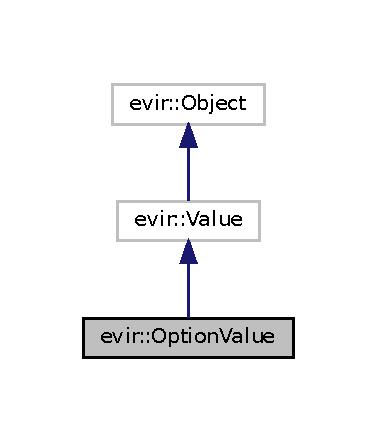
\includegraphics[width=185pt]{classevir_1_1OptionValue__inherit__graph}
\end{center}
\end{figure}


Collaboration diagram for evir\+:\+:Option\+Value\+:\nopagebreak
\begin{figure}[H]
\begin{center}
\leavevmode
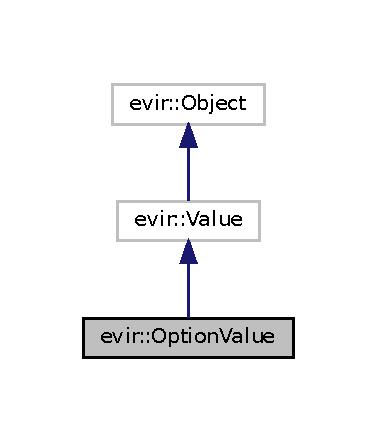
\includegraphics[width=185pt]{classevir_1_1OptionValue__coll__graph}
\end{center}
\end{figure}
\subsection*{Public Member Functions}
\begin{DoxyCompactItemize}
\item 
string \hyperlink{classevir_1_1OptionValue_a8bd21c46fc29805637eed4473f1fa371}{generate\+\_\+ir} (const char $\ast$format=nullptr)
\item 
\mbox{\Hypertarget{classevir_1_1OptionValue_aa1747703bb1bb354c6dc8c0b7d5b0766}\label{classevir_1_1OptionValue_aa1747703bb1bb354c6dc8c0b7d5b0766}} 
{\bfseries Option\+Value} (string name)
\end{DoxyCompactItemize}
\subsection*{Public Attributes}
\begin{DoxyCompactItemize}
\item 
\mbox{\Hypertarget{classevir_1_1OptionValue_a63f37acb5bd04ab6c2dd9ddb78e70318}\label{classevir_1_1OptionValue_a63f37acb5bd04ab6c2dd9ddb78e70318}} 
string {\bfseries name}
\end{DoxyCompactItemize}
\subsection*{Additional Inherited Members}


\subsection{Member Function Documentation}
\mbox{\Hypertarget{classevir_1_1OptionValue_a8bd21c46fc29805637eed4473f1fa371}\label{classevir_1_1OptionValue_a8bd21c46fc29805637eed4473f1fa371}} 
\index{evir\+::\+Option\+Value@{evir\+::\+Option\+Value}!generate\+\_\+ir@{generate\+\_\+ir}}
\index{generate\+\_\+ir@{generate\+\_\+ir}!evir\+::\+Option\+Value@{evir\+::\+Option\+Value}}
\subsubsection{\texorpdfstring{generate\+\_\+ir()}{generate\_ir()}}
{\footnotesize\ttfamily string evir\+::\+Option\+Value\+::generate\+\_\+ir (\begin{DoxyParamCaption}\item[{const char $\ast$}]{format = {\ttfamily nullptr} }\end{DoxyParamCaption})\hspace{0.3cm}{\ttfamily [virtual]}}

Generates the IR for the value \begin{DoxyReturn}{Returns}
the IR as a string (without a newline) 
\end{DoxyReturn}


Implements \hyperlink{classevir_1_1Value_a3e7e5bc634fd5bba528324076fe2a763}{evir\+::\+Value}.



The documentation for this class was generated from the following file\+:\begin{DoxyCompactItemize}
\item 
include/ir/object/value.\+hpp\end{DoxyCompactItemize}

\hypertarget{classevir_1_1ReferenceValue}{}\section{evir\+:\+:Reference\+Value Class Reference}
\label{classevir_1_1ReferenceValue}\index{evir\+::\+Reference\+Value@{evir\+::\+Reference\+Value}}


Inheritance diagram for evir\+:\+:Reference\+Value\+:\nopagebreak
\begin{figure}[H]
\begin{center}
\leavevmode
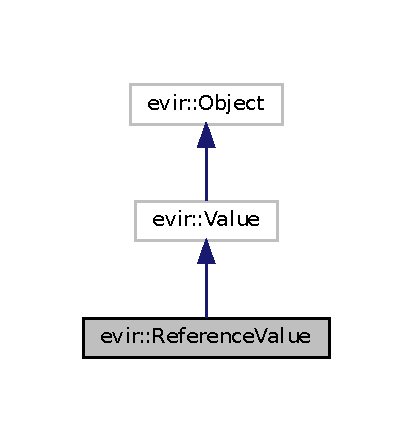
\includegraphics[width=203pt]{classevir_1_1ReferenceValue__inherit__graph}
\end{center}
\end{figure}


Collaboration diagram for evir\+:\+:Reference\+Value\+:\nopagebreak
\begin{figure}[H]
\begin{center}
\leavevmode
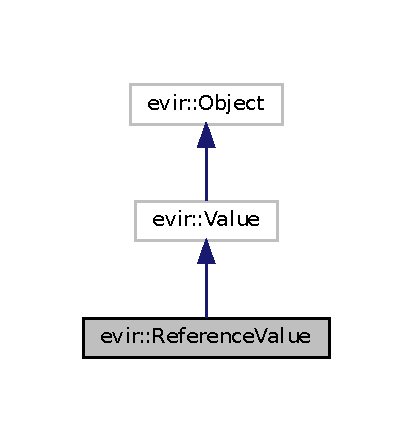
\includegraphics[width=203pt]{classevir_1_1ReferenceValue__coll__graph}
\end{center}
\end{figure}
\subsection*{Public Member Functions}
\begin{DoxyCompactItemize}
\item 
string \hyperlink{classevir_1_1ReferenceValue_ad669613befab66578629de2ccfb8c2c3}{generate\+\_\+ir} (const char $\ast$format=nullptr)
\item 
\mbox{\Hypertarget{classevir_1_1ReferenceValue_a9f20a5682fe940f5ca31cbc48ff17c84}\label{classevir_1_1ReferenceValue_a9f20a5682fe940f5ca31cbc48ff17c84}} 
{\bfseries Reference\+Value} (string name)
\end{DoxyCompactItemize}
\subsection*{Public Attributes}
\begin{DoxyCompactItemize}
\item 
\mbox{\Hypertarget{classevir_1_1ReferenceValue_ab1ee319a03944d8622ea3b06394cef1d}\label{classevir_1_1ReferenceValue_ab1ee319a03944d8622ea3b06394cef1d}} 
string {\bfseries name}
\end{DoxyCompactItemize}
\subsection*{Additional Inherited Members}


\subsection{Member Function Documentation}
\mbox{\Hypertarget{classevir_1_1ReferenceValue_ad669613befab66578629de2ccfb8c2c3}\label{classevir_1_1ReferenceValue_ad669613befab66578629de2ccfb8c2c3}} 
\index{evir\+::\+Reference\+Value@{evir\+::\+Reference\+Value}!generate\+\_\+ir@{generate\+\_\+ir}}
\index{generate\+\_\+ir@{generate\+\_\+ir}!evir\+::\+Reference\+Value@{evir\+::\+Reference\+Value}}
\subsubsection{\texorpdfstring{generate\+\_\+ir()}{generate\_ir()}}
{\footnotesize\ttfamily string evir\+::\+Reference\+Value\+::generate\+\_\+ir (\begin{DoxyParamCaption}\item[{const char $\ast$}]{format = {\ttfamily nullptr} }\end{DoxyParamCaption})\hspace{0.3cm}{\ttfamily [virtual]}}

Generates the IR for the value \begin{DoxyReturn}{Returns}
the IR as a string (without a newline) 
\end{DoxyReturn}


Implements \hyperlink{classevir_1_1Value_a3e7e5bc634fd5bba528324076fe2a763}{evir\+::\+Value}.



The documentation for this class was generated from the following file\+:\begin{DoxyCompactItemize}
\item 
include/ir/object/value.\+hpp\end{DoxyCompactItemize}

\hypertarget{classevir_1_1StringValue}{}\section{evir\+:\+:String\+Value Class Reference}
\label{classevir_1_1StringValue}\index{evir\+::\+String\+Value@{evir\+::\+String\+Value}}


Inheritance diagram for evir\+:\+:String\+Value\+:
\nopagebreak
\begin{figure}[H]
\begin{center}
\leavevmode
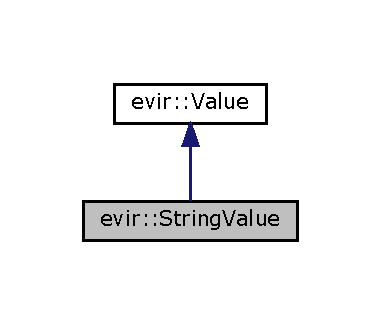
\includegraphics[width=183pt]{classevir_1_1StringValue__inherit__graph}
\end{center}
\end{figure}


Collaboration diagram for evir\+:\+:String\+Value\+:
\nopagebreak
\begin{figure}[H]
\begin{center}
\leavevmode
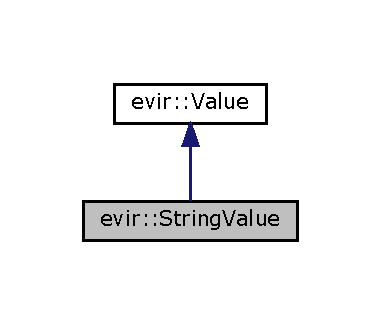
\includegraphics[width=183pt]{classevir_1_1StringValue__coll__graph}
\end{center}
\end{figure}
\subsection*{Public Member Functions}
\begin{DoxyCompactItemize}
\item 
string \hyperlink{classevir_1_1StringValue_ae635609dfe7acf237b71bdb48625712e}{generate\+\_\+ir} (const char $\ast$format=nullptr)
\item 
\mbox{\Hypertarget{classevir_1_1StringValue_a91176d5ea0ac4df11329e8a53eff3f21}\label{classevir_1_1StringValue_a91176d5ea0ac4df11329e8a53eff3f21}} 
{\bfseries String\+Value} (string value)
\end{DoxyCompactItemize}
\subsection*{Public Attributes}
\begin{DoxyCompactItemize}
\item 
\mbox{\Hypertarget{classevir_1_1StringValue_a67f645bf8d1e71c7b8239c65a795d17f}\label{classevir_1_1StringValue_a67f645bf8d1e71c7b8239c65a795d17f}} 
string {\bfseries value}
\end{DoxyCompactItemize}
\subsection*{Additional Inherited Members}


\subsection{Member Function Documentation}
\mbox{\Hypertarget{classevir_1_1StringValue_ae635609dfe7acf237b71bdb48625712e}\label{classevir_1_1StringValue_ae635609dfe7acf237b71bdb48625712e}} 
\index{evir\+::\+String\+Value@{evir\+::\+String\+Value}!generate\+\_\+ir@{generate\+\_\+ir}}
\index{generate\+\_\+ir@{generate\+\_\+ir}!evir\+::\+String\+Value@{evir\+::\+String\+Value}}
\subsubsection{\texorpdfstring{generate\+\_\+ir()}{generate\_ir()}}
{\footnotesize\ttfamily string evir\+::\+String\+Value\+::generate\+\_\+ir (\begin{DoxyParamCaption}\item[{const char $\ast$}]{format = {\ttfamily nullptr} }\end{DoxyParamCaption})\hspace{0.3cm}{\ttfamily [virtual]}}

Generates the IR for the value \begin{DoxyReturn}{Returns}
the IR as a string (without newline) 
\end{DoxyReturn}


Implements \hyperlink{classevir_1_1Value_a3e7e5bc634fd5bba528324076fe2a763}{evir\+::\+Value}.



The documentation for this class was generated from the following file\+:\begin{DoxyCompactItemize}
\item 
include/ir/value.\+hpp\end{DoxyCompactItemize}

\hypertarget{classevir_1_1Value}{}\section{evir\+:\+:Value Class Reference}
\label{classevir_1_1Value}\index{evir\+::\+Value@{evir\+::\+Value}}


Inheritance diagram for evir\+:\+:Value\+:
\nopagebreak
\begin{figure}[H]
\begin{center}
\leavevmode
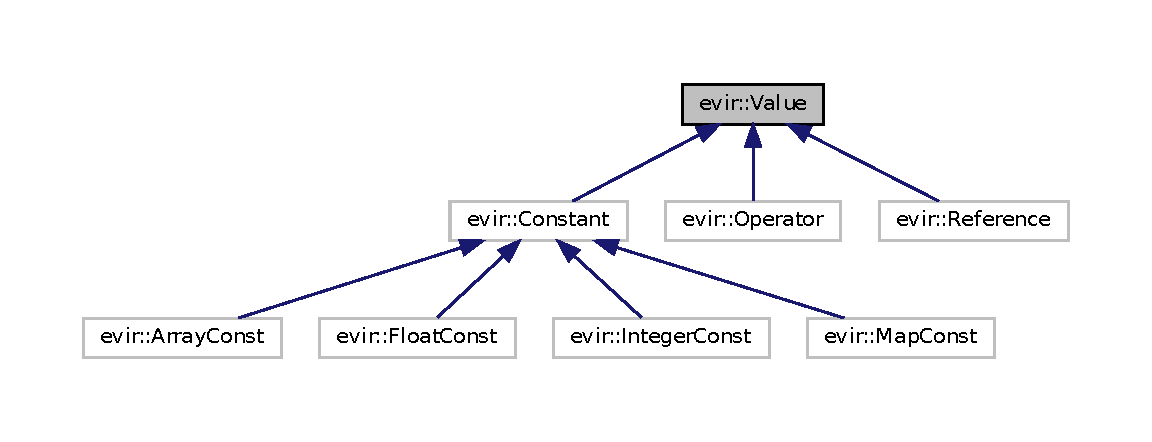
\includegraphics[width=312pt]{classevir_1_1Value__inherit__graph}
\end{center}
\end{figure}
\subsection*{Public Member Functions}
\begin{DoxyCompactItemize}
\item 
virtual string \hyperlink{classevir_1_1Value_a3e7e5bc634fd5bba528324076fe2a763}{generate\+\_\+ir} (const char $\ast$format=nullptr)=0
\end{DoxyCompactItemize}
\subsection*{Static Public Member Functions}
\begin{DoxyCompactItemize}
\item 
static \hyperlink{classevir_1_1IntegerValue}{Integer\+Value} $\ast$ \hyperlink{classevir_1_1Value_a086f7932417f5b1fa47f627c175d1c65}{new\+\_\+integer} (int64 value)
\item 
static \hyperlink{classevir_1_1FloatValue}{Float\+Value} $\ast$ \hyperlink{classevir_1_1Value_a90a29b6a33606b8ada904688ce0a302f}{new\+\_\+float} (float2 value)
\item 
static \hyperlink{classevir_1_1StringValue}{String\+Value} $\ast$ \hyperlink{classevir_1_1Value_a56a75d435ff168c8d3f104018f9b58a5}{new\+\_\+string} (string value)
\item 
static \hyperlink{classevir_1_1ListValue}{List\+Value} $\ast$ \hyperlink{classevir_1_1Value_a0936d4b3ac1b972fc784dc6b71ca0ca2}{new\+\_\+list} (vector$<$ \hyperlink{classevir_1_1Value}{Value} $\ast$$>$ elements)
\item 
static \hyperlink{classevir_1_1ObjectValue}{Object\+Value} $\ast$ \hyperlink{classevir_1_1Value_a4afc4919cf8f686d97a8f59ea7719ac1}{new\+\_\+object} (map$<$ \hyperlink{classevir_1_1Value}{Value} $\ast$C\+O\+M\+MA \hyperlink{classevir_1_1Value}{Value} $\ast$$>$ pairs)
\item 
static \hyperlink{classevir_1_1ReferenceValue}{Reference\+Value} $\ast$ \hyperlink{classevir_1_1Value_a550b2d56a46a357282ad167821fedbe5}{new\+\_\+reference} (string name)
\item 
static \hyperlink{classevir_1_1OptionValue}{Option\+Value} $\ast$ \hyperlink{classevir_1_1Value_af0e8e17cc7ab9c0907ba4c8994ef169a}{new\+\_\+option} (string name)
\end{DoxyCompactItemize}


\subsection{Member Function Documentation}
\mbox{\Hypertarget{classevir_1_1Value_a3e7e5bc634fd5bba528324076fe2a763}\label{classevir_1_1Value_a3e7e5bc634fd5bba528324076fe2a763}} 
\index{evir\+::\+Value@{evir\+::\+Value}!generate\+\_\+ir@{generate\+\_\+ir}}
\index{generate\+\_\+ir@{generate\+\_\+ir}!evir\+::\+Value@{evir\+::\+Value}}
\subsubsection{\texorpdfstring{generate\+\_\+ir()}{generate\_ir()}}
{\footnotesize\ttfamily virtual string evir\+::\+Value\+::generate\+\_\+ir (\begin{DoxyParamCaption}\item[{const char $\ast$}]{format = {\ttfamily nullptr} }\end{DoxyParamCaption})\hspace{0.3cm}{\ttfamily [pure virtual]}}

Generates the IR for the value \begin{DoxyReturn}{Returns}
the IR as a string (without newline) 
\end{DoxyReturn}


Implemented in \hyperlink{classevir_1_1OptionValue_a8bd21c46fc29805637eed4473f1fa371}{evir\+::\+Option\+Value}, \hyperlink{classevir_1_1ReferenceValue_ad669613befab66578629de2ccfb8c2c3}{evir\+::\+Reference\+Value}, \hyperlink{classevir_1_1ObjectValue_a1058f47731ab800327893e388fc2b2d0}{evir\+::\+Object\+Value}, \hyperlink{classevir_1_1ListValue_aebd962d9117d8cd22d35bf217975dcff}{evir\+::\+List\+Value}, \hyperlink{classevir_1_1StringValue_ae635609dfe7acf237b71bdb48625712e}{evir\+::\+String\+Value}, \hyperlink{classevir_1_1FloatValue_a775e25d41c34aca73ed9418963bb652b}{evir\+::\+Float\+Value}, and \hyperlink{classevir_1_1IntegerValue_a586411c365b2afc18fbd5960dd053d94}{evir\+::\+Integer\+Value}.

\mbox{\Hypertarget{classevir_1_1Value_a90a29b6a33606b8ada904688ce0a302f}\label{classevir_1_1Value_a90a29b6a33606b8ada904688ce0a302f}} 
\index{evir\+::\+Value@{evir\+::\+Value}!new\+\_\+float@{new\+\_\+float}}
\index{new\+\_\+float@{new\+\_\+float}!evir\+::\+Value@{evir\+::\+Value}}
\subsubsection{\texorpdfstring{new\+\_\+float()}{new\_float()}}
{\footnotesize\ttfamily static \hyperlink{classevir_1_1FloatValue}{Float\+Value}$\ast$ evir\+::\+Value\+::new\+\_\+float (\begin{DoxyParamCaption}\item[{float2}]{value }\end{DoxyParamCaption})\hspace{0.3cm}{\ttfamily [static]}}

Constructs a new float value 
\begin{DoxyParams}{Parameters}
{\em value} & the float \\
\hline
\end{DoxyParams}
\mbox{\Hypertarget{classevir_1_1Value_a086f7932417f5b1fa47f627c175d1c65}\label{classevir_1_1Value_a086f7932417f5b1fa47f627c175d1c65}} 
\index{evir\+::\+Value@{evir\+::\+Value}!new\+\_\+integer@{new\+\_\+integer}}
\index{new\+\_\+integer@{new\+\_\+integer}!evir\+::\+Value@{evir\+::\+Value}}
\subsubsection{\texorpdfstring{new\+\_\+integer()}{new\_integer()}}
{\footnotesize\ttfamily static \hyperlink{classevir_1_1IntegerValue}{Integer\+Value}$\ast$ evir\+::\+Value\+::new\+\_\+integer (\begin{DoxyParamCaption}\item[{int64}]{value }\end{DoxyParamCaption})\hspace{0.3cm}{\ttfamily [static]}}

Constructs a new integer value 
\begin{DoxyParams}{Parameters}
{\em value} & the integer \\
\hline
\end{DoxyParams}
\mbox{\Hypertarget{classevir_1_1Value_a0936d4b3ac1b972fc784dc6b71ca0ca2}\label{classevir_1_1Value_a0936d4b3ac1b972fc784dc6b71ca0ca2}} 
\index{evir\+::\+Value@{evir\+::\+Value}!new\+\_\+list@{new\+\_\+list}}
\index{new\+\_\+list@{new\+\_\+list}!evir\+::\+Value@{evir\+::\+Value}}
\subsubsection{\texorpdfstring{new\+\_\+list()}{new\_list()}}
{\footnotesize\ttfamily static \hyperlink{classevir_1_1ListValue}{List\+Value}$\ast$ evir\+::\+Value\+::new\+\_\+list (\begin{DoxyParamCaption}\item[{vector$<$ \hyperlink{classevir_1_1Value}{Value} $\ast$$>$}]{elements }\end{DoxyParamCaption})\hspace{0.3cm}{\ttfamily [static]}}

Constructs a new list value 
\begin{DoxyParams}{Parameters}
{\em elements} & the elements of the list \\
\hline
\end{DoxyParams}
\mbox{\Hypertarget{classevir_1_1Value_a4afc4919cf8f686d97a8f59ea7719ac1}\label{classevir_1_1Value_a4afc4919cf8f686d97a8f59ea7719ac1}} 
\index{evir\+::\+Value@{evir\+::\+Value}!new\+\_\+object@{new\+\_\+object}}
\index{new\+\_\+object@{new\+\_\+object}!evir\+::\+Value@{evir\+::\+Value}}
\subsubsection{\texorpdfstring{new\+\_\+object()}{new\_object()}}
{\footnotesize\ttfamily static \hyperlink{classevir_1_1ObjectValue}{Object\+Value}$\ast$ evir\+::\+Value\+::new\+\_\+object (\begin{DoxyParamCaption}\item[{map$<$ \hyperlink{classevir_1_1Value}{Value} $\ast$C\+O\+M\+MA \hyperlink{classevir_1_1Value}{Value} $\ast$$>$}]{pairs }\end{DoxyParamCaption})\hspace{0.3cm}{\ttfamily [static]}}

Constructs a new object value 
\begin{DoxyParams}{Parameters}
{\em pair} & the key-\/value pairs of the object \\
\hline
\end{DoxyParams}
\mbox{\Hypertarget{classevir_1_1Value_af0e8e17cc7ab9c0907ba4c8994ef169a}\label{classevir_1_1Value_af0e8e17cc7ab9c0907ba4c8994ef169a}} 
\index{evir\+::\+Value@{evir\+::\+Value}!new\+\_\+option@{new\+\_\+option}}
\index{new\+\_\+option@{new\+\_\+option}!evir\+::\+Value@{evir\+::\+Value}}
\subsubsection{\texorpdfstring{new\+\_\+option()}{new\_option()}}
{\footnotesize\ttfamily static \hyperlink{classevir_1_1OptionValue}{Option\+Value}$\ast$ evir\+::\+Value\+::new\+\_\+option (\begin{DoxyParamCaption}\item[{string}]{name }\end{DoxyParamCaption})\hspace{0.3cm}{\ttfamily [static]}}

Constructs a new option value 
\begin{DoxyParams}{Parameters}
{\em name} & the name of the option \\
\hline
\end{DoxyParams}
\mbox{\Hypertarget{classevir_1_1Value_a550b2d56a46a357282ad167821fedbe5}\label{classevir_1_1Value_a550b2d56a46a357282ad167821fedbe5}} 
\index{evir\+::\+Value@{evir\+::\+Value}!new\+\_\+reference@{new\+\_\+reference}}
\index{new\+\_\+reference@{new\+\_\+reference}!evir\+::\+Value@{evir\+::\+Value}}
\subsubsection{\texorpdfstring{new\+\_\+reference()}{new\_reference()}}
{\footnotesize\ttfamily static \hyperlink{classevir_1_1ReferenceValue}{Reference\+Value}$\ast$ evir\+::\+Value\+::new\+\_\+reference (\begin{DoxyParamCaption}\item[{string}]{name }\end{DoxyParamCaption})\hspace{0.3cm}{\ttfamily [static]}}

Constructs a new reference value 
\begin{DoxyParams}{Parameters}
{\em name} & the name of the reference \\
\hline
\end{DoxyParams}
\mbox{\Hypertarget{classevir_1_1Value_a56a75d435ff168c8d3f104018f9b58a5}\label{classevir_1_1Value_a56a75d435ff168c8d3f104018f9b58a5}} 
\index{evir\+::\+Value@{evir\+::\+Value}!new\+\_\+string@{new\+\_\+string}}
\index{new\+\_\+string@{new\+\_\+string}!evir\+::\+Value@{evir\+::\+Value}}
\subsubsection{\texorpdfstring{new\+\_\+string()}{new\_string()}}
{\footnotesize\ttfamily static \hyperlink{classevir_1_1StringValue}{String\+Value}$\ast$ evir\+::\+Value\+::new\+\_\+string (\begin{DoxyParamCaption}\item[{string}]{value }\end{DoxyParamCaption})\hspace{0.3cm}{\ttfamily [static]}}

Constructs a new string value 
\begin{DoxyParams}{Parameters}
{\em value} & the string \\
\hline
\end{DoxyParams}


The documentation for this class was generated from the following file\+:\begin{DoxyCompactItemize}
\item 
include/ir/value.\+hpp\end{DoxyCompactItemize}

%--- End generated contents ---

% Index
\backmatter
\newpage
\phantomsection
\clearemptydoublepage
\addcontentsline{toc}{chapter}{Index}
\printindex

\end{document}
